%%**************************************************************
%% Vorlage fuer Bachelorarbeiten (o.ä.) der DHBW
%%
%% Autor: Tobias Dreher, Yves Fischer
%% Datum: 06.07.2011
%%
%% Autor: Michael Gruben
%% Datum: 15.05.2013
%%**************************************************************

\documentclass[%
	pdftex,
	oneside,		% Einseitiger Druck.
	12pt,			% Schriftgroesse
	parskip=half,	% Halbe Zeile Abstand zwischen Absätzen.
	headsepline,	% Linie nach Kopfzeile.
	footsepline,	% Linie vor Fusszeile.
	abstracton,	    % Abstract Überschriften
	ngerman,		% Translator
]{scrreprt}

%!TEX root = ../dokumentation.tex

%
% Nahezu alle Einstellungen koennen hier getaetigt werden
%

%Seitengroesse
\usepackage{fullpage}

%Zeilenumbruch und mehr
\usepackage[activate]{microtype}

% Zeichencodierung
\usepackage[utf8]{inputenc}
\usepackage[T1]{fontenc}

% Zeilenabstand
\usepackage[onehalfspacing]{setspace}

% Index-Erstellung
\usepackage{makeidx}

% Lokalisierung (neue deutsche Rechtschreibung)
\usepackage[ngerman]{babel}

% Anführungszeichen 
\usepackage[babel,german=quotes]{csquotes}
%\usepackage[style=swiss]{csquotes}


% Spezielle Tabellenform fuer Deckblatt
\usepackage{longtable}
\setlength{\tabcolsep}{10pt} %Abstand zwischen Spalten
\renewcommand{\arraystretch}{1.5} %Zeilenabstand

% Grafiken
\usepackage{graphicx}

% Mathematische Textsaetze
%\usepackage{amsmath}
%\usepackage{amssymb}

% Pakete um Textteile drehen zu können, oder eine Seite Querformat anzeigen kann.
%\usepackage{rotating}
%\usepackage{lscape}

% Farben
\usepackage{color}
\definecolor{LinkColor}{rgb}{0,0,0.2}
\definecolor{ListingBackground}{rgb}{0.92,0.92,0.92}

\newcommand{\pdftitel}{Entwicklung einer Auto-Dashboard-Applikation zur berührungslosen Interaktion im Straßenverkehr}
\newcommand{\aram}{Aram Parsegyan}
\newcommand{\fabian}{Fabian Schäfer}
\newcommand{\arbeit}{Studienarbeit}

% Titel, Autor und Datum
\title{\titel}
\author{\autor}
\date{\datum}

% PDF Einstellungen
\usepackage[%
	pdftitle={\pdftitel},
	pdfauthor={\autor},
	pdfsubject={\arbeit},
	pdfcreator={pdflatex, LaTeX with KOMA-Script},
	pdfpagemode=UseOutlines, % Beim Oeffnen Inhaltsverzeichnis anzeigen
	pdfdisplaydoctitle=true, % Dokumenttitel statt Dateiname anzeigen.
	pdflang=de % Sprache des Dokuments.
]{hyperref} 
    
% (Farb-)einstellungen für die Links im PDF
\hypersetup{%
	colorlinks=true, % Aktivieren von farbigen Links im Dokument
	linkcolor=LinkColor, % Farbe festlegen
	citecolor=LinkColor,
	filecolor=LinkColor,
	menucolor=LinkColor,
	urlcolor=LinkColor,
	bookmarksnumbered=true % Überschriftsnummerierung im PDF Inhalt anzeigen.
}

% Literaturverweise nach Harvard (mit deutschem und)
\usepackage[dcucite]{harvard}
\renewcommand{\harvardand}{und}
\usepackage[citestyle=reading,bibstyle=authortitle,backend=biber]{biblatex}
\addbibresource{ArbeitBib.bib}

% Verschiedene Schriftarten
%\usepackage{goudysans}
%\usepackage{lmodern}
%\usepackage{libertine}
\usepackage{palatino} 

% Hurenkinder und Schusterjungen verhindern
% http://projekte.dante.de/DanteFAQ/Silbentrennung
\clubpenalty=10000
\widowpenalty=10000
\displaywidowpenalty=10000

% Quellcode
\usepackage{listings}
\lstloadlanguages{Java}
\lstset{%
	language=Xml,		 	 % Sprache des Quellcodes
	%numbers=left,           % Zelennummern links
	stepnumber=1,            % Jede Zeile nummerieren.
	numbersep=5pt,           % 5pt Abstand zum Quellcode
	numberstyle=\tiny,       % Zeichengrösse 'tiny' für die Nummern.
	breaklines=true,         % Zeilen umbrechen wenn notwendig.
	breakautoindent=true,    % Nach dem Zeilenumbruch Zeile einrücken.
	postbreak=\space,        % Bei Leerzeichen umbrechen.
	tabsize=2,               % Tabulatorgrösse 2
	basicstyle=\ttfamily\footnotesize, % Nichtproportionale Schrift, klein für den Quellcode
	showspaces=false,        % Leerzeichen nicht anzeigen.
	showstringspaces=false,  % Leerzeichen auch in Strings ('') nicht anzeigen.
	extendedchars=true,      % Alle Zeichen vom Latin1 Zeichensatz anzeigen.
	captionpos=b,            % sets the caption-position to bottom
	backgroundcolor=\color{ListingBackground} % Hintergrundfarbe des Quellcodes setzen.
}
\lstset{literate=%
  {Ö}{{\"O}}1
  {Ä}{{\"A}}1
  {Ü}{{\"U}}1
  {ß}{{\ss}}2
  {ü}{{\"u}}1
  {ä}{{\"a}}1
  {ö}{{\"o}}1
}

% Glossar
\usepackage[
	nonumberlist, %keine Seitenzahlen anzeigen
	%acronym,      %ein Abkürzungsverzeichnis erstellen
	%section,     %im Inhaltsverzeichnis auf section-Ebene erscheinen
	toc,          %Einträge im Inhaltsverzeichnis
]{glossaries}

%Akronyme
\usepackage[printonlyused]{acronym}

% Fussnoten
\usepackage[perpage, hang, multiple, stable]{footmisc}

%Bildpfad
\graphicspath{{images/}}

%nur ein latex-Durchlauf für die Aktualisierung von Verzeichnissen nötig
\usepackage{bookmark}

%Gleitumgebungen (Bilder, Tabellen, usw\ldots) lassen sich mit H an genau der
% definierten Stelle platzieren
\usepackage{float}

% für die vertikale Platzierung von Text in Tabellen
\usepackage{array}

% für die Darstellung des Euro-Symbols
\usepackage[right]{eurosym}

% für textumflossene Grafiken
\usepackage{wrapfig}

% eine Kommentarumgebung "k" (Handhabe mit \begin{k}<Kommentartext>\end{k},
% Kommentare werden rot gedruckt). Wird \% vor excludecomment{k} entfernt,
% werden keine Kommentare mehr gedruckt.
\usepackage{comment}
\specialcomment{k}{\begingroup\color{red}}{\endgroup}
%\excludecomment{k}

\usepackage{footnote}
\makesavenoteenv{figure}


% Ab jetzt können auch Umlaute verwendet werden

%falls pdftitel = titel der Arbeit
\newcommand{\titel}{\pdftitel}
%bei unterschiedlichen Titeln
%\newcommand{\titel}{In der Regel haben wir einen zweizeiligen
% Bachelorthesistitel}
\newcommand{\martrikelnrAram}{7816495}
\newcommand{\martrikelnrFabian}{2031949}
\newcommand{\kurs}{TINF14B2}
\newcommand{\datumAbgabe}{Mai 2017}
\newcommand{\abgabeort}{Karlsruhe}
\newcommand{\abschluss}{Bachelor of Science}
\newcommand{\studiengang}{Studienganges Angewandte Informatik}
\newcommand{\dhbw}{Karlsruhe}
\newcommand{\betreuer}{Prof. Kay Berkling, PhD}
\newcommand{\zeitraum}{24 Wochen}
\newcommand{\arbeitsart}{\arbeit}

\makeglossaries
%!TEX root = ../dokumentation.tex

%
% vorher in Konsole folgendes aufrufen: 
%	makeglossaries makeglossaries dokumentation.acn && makeglossaries dokumentation.glo
%

%
% Glossareintraege --> referenz, name, beschreibung
% Aufruf mit \gls{...}
%
\newglossaryentry{Wearables}{name={Wearables},plural={Wearables},description={''Smart Wearables sind intelligente Kleinstsysteme, die in Alltagsgegenstände eingebettet sind und am Körper getragen werden. Durch die integrierten Kleinstsysteme mutieren diese Gegenstände zu intelligenter Kleidung, Smart Shoes, intelligenten Armbändern, Smartwatches, Smart Glasses oder Wearable Cameras."\footcite[][]{wearables}}}


\begin{document}

	% Deckblatt
	\begin{spacing}{1}
		%!TEX root = ../dokumentation.tex

\begin{titlepage}
	\begin{longtable}{p{.4\textwidth} p{.4\textwidth}}
	  {
\includegraphics[height=2.6cm]{images/dhbw.png}}
	\end{longtable}
	\enlargethispage{20mm}
	\begin{center}
	  \vspace*{12mm}	{\LARGE\bf \titel }\\
	  \vspace*{12mm}	{\large\bf \arbeit}\\
	  \vspace*{12mm}	für die Prüfung zum\\
	  \vspace*{3mm} 	{\bf \abschluss}\\
	  \vspace*{12mm}	des \studiengang\\
	  \vspace*{3mm} 	an der Dualen Hochschule Baden-Württemberg \dhbw\\
	  \vspace*{12mm}	von\\
	  \vspace*{3mm} 	{\large\bf \aram\ und \fabian}\\
	  \vspace*{12mm}	\datumAbgabe\\
	\end{center}
	\vfill
	\begin{spacing}{1.2}
	\begin{tabbing}
		mmmmmmmmmmmmmmmmmmmmmmmmmm     \= \kill
		\textbf{Bearbeitungszeitraum}  \>  \zeitraum\\
		\textbf{Matrikelnummern, Kurs}  \>  \martrikelnrAram, \martrikelnrFabian, \kurs\\
		%\textbf{Ausbildungsfirma}      \>  \firma, \firmenort\\
		\textbf{Betreuer}              \>  \betreuer
	\end{tabbing}
	\end{spacing}
\end{titlepage}

	\end{spacing}
	\newpage

	\renewcommand{\thepage}{\Roman{page}}
	\setcounter{page}{1}

	% Sperrvermerk
	%!TEX root = ../dokumentation.tex

\thispagestyle{empty}
% Sperrvermerk direkt hinter Titelseite
\section*{Sperrvermerk}

\vspace*{2em}

Die vorliegende {\arbeitsart} mit dem Titel {\itshape \titel} ist mit einem Sperrvermerk versehen und wird ausschließlich zu Prüfungszwecken am Studiengang {\studiengang} der Dualen Hochschule Baden-Württemberg {\abgabeort} vorgelegt.
Jede Einsichtnahme und Veröffentlichung – auch von Teilen der Arbeit – bedarf der vorherigen Zustimmung durch die Dualen Hochschule Baden-Württemberg \dhbw.

	\newpage
	
	% Erklärung
	%!TEX root = ../dokumentation.tex

\thispagestyle{empty}

\section*{Erklärung zur Eigenleistung}
% http://www.se.dhbw-mannheim.de/fileadmin/ms/wi/dl_swm/dhbw-ma-wi-organisation-bewertung-bachelorarbeit-v2-00.pdf
\vspace*{2em}

Wir versichern hiermit, dass wir unsere {\arbeitsart} mit dem Thema
{\itshape \titel } selbstständig verfasst und keine anderen als die angegebenen Quellen und Hilfsmittel benutzt haben.


Wir versichern zudem, dass die eingereichte elektronische Fassung mit der gedruckten Fassung übereinstimmt.*

{\tiny * falls beide Fassungen gefordert sind}
\vspace{2em}

\begin{tabbing}
		mmmmmmmmmmmmmmmmmmmmmmmmmm     \= \kill
        \abgabeort, \datumAbgabe  \>
        ------------------------------------\\		
		\>  Unterschrift
	\end{tabbing}

	\newpage

	% Abstract
	%!TEX root = ../dokumentation.tex

\pagestyle{empty}

\renewcommand{\abstractname}{Zusammenfassung}
\begin{abstract}
In unserer heutigen Welt spielt Kommunikation eine immer größer werdende Rolle, weshalb Smartphones aus unserem Leben nicht mehr wegzudenken sind. Als Konsequenz dieser Abhängigkeit, findet das Smartphone auch im Straßenverkehr immer häufiger Verwendung. Durch Nutzung während der Führung eines Kraftfahrzeuges wird das Unfallrisiko drastisch erhöht. Um die Zahl der somit verursachten Unfälle zu minimieren wird im Laufe dieser Arbeit eine Dashboard Applikation entwickelt. Mithilfe des Dashboardes soll der Fokus wieder auf den Straßenverkehr gelenkt werden. Zur Reduzierung des Unfallrisikos bei der Bedienung eines Smartphones wird in dieser Studienarbeit der Einsatz eines Dashboardes diskutiert. Das Dashboard soll die herkömmliche Bedienung über Berührungen durch Interaktion mittels Sprachbefehle ablösen. 

\end{abstract}


\renewcommand{\abstractname}{Summary}
\begin{abstract}
We live in a world, wherein communication plays an increasingly important role which is why it is not possible to imagine our life without smartphones. As a consequence of this dependency, the smartphone is also used more and more frequently in road traffic. Because of this usage while driving a car, the risk of an accident is drastically increased. To reduce the number of accidents caused by distractions, a dashboard application will be developed during this project, which redirects the drivers focus back to the road. This redirection will be realized by the idea of touchless interaction. Therefore interaction using voice commands replaces the common interaction of smartphones via touch.
\end{abstract}

	\newpage

	\pagestyle{plain}

	% Inhaltsverzeichnis
	\begin{spacing}{1.1}
		\setcounter{tocdepth}{1}
		%für die Anzeige von Unterkapiteln im Inhaltsverzeichnis
		\setcounter{tocdepth}{2}
		\tableofcontents
	\end{spacing}
	\newpage

	\renewcommand{\thepage}{\arabic{page}}
	\setcounter{page}{1}
	
	% Inhalt
	%!TEX root = ../dokumentation.tex

\chapter{Einleitung}
In unserer heutigen Welt gibt es einen stetigen Anstieg der weltweiten Bevölkerung. Parallel zu diesem, steigt auch die Anzahl der Kraftfahrzeuge.
Wegen stetiger Zunahme der Verkehrsteilnehmer und der Häufigkeit von Fahrten besteht eine höher werdende Wahrscheinlichkeit einen Unfall auf dem Weg von Startpunkt A nach Zielpunkt B zu haben. Unfallfreies bewegen mit dem Kraftfahrzeug fordert die volle Konzentration des Fahrzeugführers für den Straßenverkehr. Jede Ablenkung vom Straßenverkehr führt zu einem ansteigen des Unfallrisikos.
Laut Statistik sind mehr als 33 Prozent der Unfälle auf Ablenkungen zurückzuführen.
Dabei nehmen Smartphones einen immer größer werdenden Teil in dieser Statistik ein, insbesondere bei Fahrern zwischen 18 und 24. Ablenkung durch Smartphones können beispielsweise durch eine eingehende Benachrichtigungen, beantworten von Telefongesprächen ohne Freisprecheinrichtung oder durch manuelle Bedienung verursacht werden.\footcite[vgl.:][]{heiseAblenkungSmartphone}

Ziel dieser Arbeit ist es, die Ablenkungen im Straßenverkehr, die durch die Interaktion mit dem Smartphone entstehen, auf ein Minimum zu reduzieren und somit das Unfallrisiko durch Ablenkungen zu senken. Dies soll durch die Verwendung einer Applikation namens \ac{ANNA} umgesetzt werden. Die Idee ist, die Interaktion mit dem Smarthpone durch Berührungen komplett auf Sprachsteuerung umzustellen und abzulösen. Wegen dem wegfallen der manuellen Bedienung kann sich der Fahrer besser auf den Straßenverkehr konzentrieren. Durch diese Umverteilung des Fokus wird Fahrern eine Applikation geboten, die es ihnen ermöglicht, auch während der Fahrt mit anderen Personen zu kommunizieren, ohne das eigene Unfall Risiko drastisch zu erhöhen.

\section{Motivation}
Das Projekt \ac{ANNA} basiert auf der Idee einen Fahrassistenten, wie er bereits in zahlreichen Oberklasse Fahrzeugen enthalten ist, für jeden zugänglich zu machen. Ziel dieses Assistenten ist es, die manuelle Interaktion mit einem Smartphone zu vermeiden. Die Erwartung ist, den Anteil der Verkehrsunfälle, die auf Ablenkungen durch das Smartphone zurückzuführen sind, zu minimieren.

Gerade jüngere Menschen sind von einer Ablenkung stärker betroffen. Das Smartphone nimmt einen wichtigeren Teil ihres Lebens ein, als es bei älteren Menschen der Fall ist. Außerdem sind jüngere Menschen noch nicht so erfahren im Straßenverkehr, woraus ohnehin ein höheres Unfallrisiko entsteht.
Oberklasse Fahrzeuge zielen mit ihren Assistenten eigentlich auf die falsche Nutzergruppe ab. Ältere Menschen, welche sich ein Oberklasse Auto leisten können, nutzen ihr Smartphone meist nicht so häufig wie jüngere Menschen. Außerdem haben sie mehr Erfahrungen im Straßenverkehr wodurch insgesamt das Unfallrisiko niedriger ist.\\
Das Projekt \ac{ANNA} zielt eher auf jüngere Nutzer ab, welche einen Fahrassistenten wirklich brauchen, um so die Anzahl der Unfälle durch Ablenkung von Smartphones zu minimieren.

Die starke Einschränkung, der in Oberklasse Fahrzeugen verbauten Systeme, ist ein ausschlaggebender Punkt für die Entwicklungsidee von \ac{ANNA}.\\
Die Interaktion dieser Systeme ist meist auf Basisfunktionen, wie z.B. Telefonanrufe, SMS und Navigation beschränkt.\\
Durch einen Fahrassistent der hingegen direkt auf dem Smartphone arbeitet und nicht nur über Bluetooth mit dem Smartphone verbunden ist, bieten sich viel weitreichendere Möglichkeiten zur Interaktion mit anderen Funktionen. So können beispielsweise verschiedene Messenger verwendet werden anstatt nur SMS oder auch mit der favorisierten Musikplayer App interagiert werden.

\section{Problemstellung}
Ein wichtiger Aspekt bei der Entwicklung von \ac{ANNA} ist die Modularität. Die App soll keine Funktionen beinhalten, die der jeweilige Nutzer nicht nutzt. Daher werden beim initialen Start der App alle installierten Apps auf dem Smartphone gescannt, um schließlich dem Nutzer nur die für ihn relevanten Module anzuzeigen. Der Nutzer kann anschließend selbst entscheiden, welche Funktionalitäten er in seinen Fahrassistent aufnehmen will.

Ein weiterer wichtiger Punkt ist die Interaktion mit anderen Anwendungen. Nicht alle Anwendungen bieten eine \ac{API} an, um über diese mit der jeweiligen Anwendung zu interagieren. Vor allem Messenger Dienste wie z.B. WhatsApp sehen keine Interaktion durch dritte mit ihrem Dienst vor. Um diese Problematik zu lösen, müssen die einzelnen Anwendungen und ihr Funktionsweisen analysiert werden, um aus diesen Funktionsweisen Schlüsse, zur Implementierung von Interaktionen auf reiner Geräteebene, zu ziehen.

In Hinblick auf die Interaktion im Fahrzeug, ergibt sich bei der Spracherkennungsfunktion folgendes Problem: Zwischen dem Nutzer und dem Mikrofon zur Erkennung des gesprochenen Worts liegt in der Regel eine mittlere Distanz, da das Smartphone meist in einer Halterung nahe der Windschutzscheibe platziert wird. Außerdem entstehen durch die Geräuschkulisse  des Straßenverkehrs Störgeräusche, welche die Sprachanalyse erschweren.\\
Um dem Problem entgegenzuwirken, muss eine gewisse Fehlertoleranz bei der Analyse des gesprochenen Wortes berücksichtigt werden.\\
Zur Gewinnung weiterer Erkenntnisse, in Hinblick auf das verwendete Mikrofon, werden im weiteren Verlauf dieser Arbeit entsprechende Untersuchungen durchgeführt.

\section{Anforderungen}
\label{sec:requirements}
Bei der Projektidee, einen Oberklasse Fahrassistenten für jeden verfügbar zu machen, dient das mobile Betriebssystem Android als Basis. Durch die Wahl von Android als Basisbetriebssystems, ist es möglich 87,5\% der weltweiten Smartphonenutzer zu erreichen.\footcite[vgl.:][]{t3n}  

Um Nutzern mit einer älteren Androidversion von der Verwendung von \ac{ANNA} nicht auszuschließen, wird Kitkat 4.4 als älteste Version des Betriebssystems unterstützt. Somit werden 86,7\% (Stand: Februar 2017) der Androidnutzer erreicht.\footcite[vgl.:][]{androidDistribution}

Um das Ziel zu verwirklichen, den Straßenverkehr sicherer zu gestalten, wird die App kostenlos zur Verfügung gestellt, um somit keine potentiellen Nutzer durch eine Kaufgebühr abzuschrecken. Ein weiter Punkt um dieses Ziel umzusetzen besteht darin, die aktive Interaktion mit der Smartphone durch Berührungseingaben und aktives Lesen zu vermeiden. Hierzu werden eingehende Benachrichtigungen vorgelesen und der Nutzer kann mit dem System durch reine Sprachbefehle interagieren.

Der Nutzer mit seinen Bedürfnissen steht bei der Entwicklung von \ac{ANNA} im Vordergrund. Die Privatsphäre des Nutzers geschützt, indem Audioaufnahmen zur weiteren Verarbeitung nicht an für den Nutzer unzugängliche Server geschickt werden, sondern direkt auf dem Endgerät verarbeitet werden. Dies schützt nicht nur die Privatsphäre, sondern spart auch Datenvolumen des Nutzers.
Die von \ac{ANNA} vorgelesenen Benachrichtigungen werden nicht gespeichert oder für andere Zwecke als der Interaktion mit dem Nutzer der App verwendet.

Neben der Privatsphäre der Nutzer steht ebenso die Individualität der Nutzer im Vordergrund. Da unterschiedliche Nutzergruppen unterschiedliche Applikationen wie z.B. verschiedene Messenger-, Karten- oder Musikdienste nutzen, sollte auch ihr Fahrassistent individuell konfigurierbar sein. Zu diesem Zweck kann der Nutzer aus einer Liste verschiedene Module für seinen Fahrassistenten auswählen.

Ein weiterer Schwerpunkt bei der Entwicklung von \ac{ANNA} liegt im Design der Benutzeroberfläche. Hierzu orientiert sich das Aussehen an dem von Google definierten Material-Design, welches in den aktuellen Versionen des Betriebssystems Android Einzug hält und das vorhergehende Holo-Design ablöst.


	%!TEX root = ../dokumentation.tex

\chapter{Konzeption}
In den Nachfolgenden Sektionen werden die grundlegenden Technologien und Geräte beschrieben, welche für die Umsetzung dieses Projekts verwendet werden sowie entsprechende Alternativen. Außerdem werden bereits auf dem Markt vorhandene Applikationen mit ähnlichen Funktionsumfang analysiert und deren Stärken und Schwächen herausgearbeitet.\\
Die Analysen beziehen sich hierbei auf die für das Projekt ANNA festgelegten Ziele.

\section{Speech API}
Für die Sprachausgabe sowie vor allem auch für die Spracherkennung, welche zur Interaktion mit der Applikation dienen soll, ist es erforderlich sich mit den zahlreichen vorhandenen Speech APIs auseinander zu setzen, um so die geeignetste für dieses Projekt herauszufiltern.

Der Prozess der Umwandlung des gesprochenen Worts in die geschriebene Form wird als decoding bezeichnet.\\
Die Theorie der Linguistik beschreibt Sprache durch Phonetik, Phonologie, Morphonologie, Syntax, Semantik und Pragmatik. Vor allem die ersten vier dieser Punkte werden von Frameworks zur Umwandlung von Sprache in Text verwendet. Dabei wird versucht das beste Ergebnis durch die Kombination der höchsten Trefferrate der einzelnen Aspekte, durch die Sprache beschrieben wird, zu finden.\\
Die meisten modernen Spracherkennungssysteme nutzen statistische Methoden und maschinelles Lernen zur Verbesserung der von ihnen genutzten Aspekte, welche zur Beschreibung der Sprache verwendet werden.\footcite[vgl.:][]{CMUSphinx} \footcite[vgl.:][S. 410 f]{automaticSpeechRecognition}

In den Nachfolgenden Kapiteln werden insgesamt fünf Speech \ac{API}s untersucht und eine Übersicht über deren Vor- und Nachteile gegeben.

\subsection{Voice Action}
Bei \ac{VA}, welches von Google entwickelt wird, handelt es sich um das standardmäßig mit dem, für mobile Geräte entwickelte Betriebssystem, Android bereitgestelltem Framework zur auditiven Kommunikation zwischen Anwender und System.

Der offensichtlichste Vorteil bei dieser \ac{API} besteht darin, dass sei von Google selbst gepflegt wird und standardmäßig auf Android Geräten verfügbar ist. Da die Applikation so kein eigenes Sprachframework mitliefern muss, wird der Speicherverbrauch entsprechend minimiert.\\
Des Weiteren ergibt sich durch die Verwendung der \ac{VA} \ac{API} die Möglichkeit die eigene Applikation in den Funktionsumfang des von Google bereitgestellten Sprachassistenten ,,Google Now'' zu integrieren. Ein einfaches Beispiel an dieser Stelle wäre eine Wecker-Applikation.\\
Durch die Einbindung von \ac{VA}, wäre es hier möglich, dass die Wecker-Applikation in den Funktionsumfang von Google Now integriert wird, dass wenn ein mit Google Now interagierender Nutzer den Befehl ,,Ok Goole, stelle einen Wecker auf 8 Uhr!'' nutzt, die hier beschriebene Wecker-Applikation von Google Now angesprochen wird um diese Aktion durchzuführen, anstatt den vorinstallierten System-Wecker zu verwenden.\footcite[vgl.:][]{voiceActions}

Der Nachteil bei der Verwendung von \ac{VA} besteht in dem geringen Funktionsumfang für den Entwickler.\\
Dem Entwickler stehen im Wesentlichen nur die Funktionen zur Text in Sprache sowie zur Sprache in Text Umwandlung zur Verfügung. Alle weiteren Verarbeitungsschritte innerhalb dieser Methoden können nicht durch den Entwickler verändert werden um sie so an die jeweiligen Situationen anzupassen.\\
Ein weiterer Nachteil bei der Verwendung von \ac{VA} besteht darin, dass sich die Nutzung auf Android-Geräte begrenzt und es somit nicht möglich ist, es auch für andere Betriebssysteme zu verwenden.\footcite[vgl.:][]{voiceActions}

\ac{VA} bietet für die Berechnung und Umwandlung der Spracheingaben die Möglichkeit die Umwandlung in Text rein auf dem Gerät ausführen zu lassen, jedoch muss dies explizit durch den Nutzer eingestellt werden. Standardmäßig werden die Spracheingaben an Server von Google gesendet um dort verarbeitet zu werden und das Resultat zurück an das entsprechende Gerät gesendet. Zusätzlich wird bei der serverseitigen Verarbeitung eine Kopie der Spracheingabe gespeichert, welche so lange existieren bleibt bis der Nutzer diese eigenständig über eine entsprechende Webseite löscht.\footcite[vgl.:][]{voiceActions}

\subsection{Siri}
Apples Sprachassistent, Siri, bietet seit 2011 die Möglichkeit mit seinem Smartphones und Tablets berührungslos zu interagieren. Allerdings müssen die Geräte ausnahmslos von Apple stammen, um Siri benutzen zu können.\footcite[vgl.:][]{Siriexplained} 

Durch die Entwicklung von Siri weggehend von einem seperaten Modul und hin zu einer stärkeren Intergriergung des Assistenten in das Firmen eigene Betriebssystem, wurde ein großer Fortschritt in Richtung maschineller Unterstützung erzielt. Ab diesem konnte Siri schneller und einfacher mit Apple eigenen Services kommunizieren, welche später noch durch viele weitere externe Services wie Yelp, Rotten Tomatoes, Shazam und einiger anderer online Services ergänzt wurden. Durch die Anbindung all dieser Dienste ist Siri in der Lage noch gezieltere und genauere Antworten auf eingehende Fragen zu geben.\footcite[vgl.:][]{appleSiri} \footcite[vgl.:][]{Siriexplained} 

Dabei hangelt sich Siri an verschiedenen Schritten lang, um das Gesprochene zu erkennen.
Zuerst wird die Stimme in eine kompakte digitale Form umgewandelt. Danach wird ausgewertet, ob der Befehl direkt auf dem Smartphone, also lokal, oder in der Cloud erledigt werden soll. Eingaben wie ,,Spiele einen Song aus meiner Mediathek'' wird lokal ausgeführt. Alle anderen Befehle, welche Zugriff auf das Internet benötigen, werden in der Cloud berechnet. Gleichzeitig wird sowohl lokal auf dem Smartphone als auch auf dem Server das Gesprochene im digitalen Format gegen verschiedenen Statistische Modelle geprüft um herauszufinden, welche Buchstaben benutzt wurden. Derjenige von beiden, welcher eine höhere Wahrscheinlichkeit ausgibt, gibt sein Ergebnis an ein Sprach Modell, welches dann abschätzt welche Wörter gesagt wurden und danach den Befehl ausführen. Wenn sich Siri zu unsicher ist fragt sie jedoch erneut nach.\footcite[vgl.:][]{howSiriWork}

Heute funktioniert Siri mit nahezu allen Apple Produkten, welche ein Mikrofon besitzen. Dennoch schränkt Apple die Benutzung des Services mit nur IOS fähigen Geräten drastisch ein. Dennoch wurde Siri 2016 erstmals für den Zugriff von Drittanbietern Software geöffnet. Wodurch sich Siri erstmals als Assistent für verschiedene Applikationen seit ihrer Entwicklung anbietet.\footcite[vgl.:][]{appleSiri}\footcite[vgl.:][]{Siriexplained}

\subsection{Alexa}
Das Spracherkennungssystem Alexa Voice Services, kurz Alexa, ist der Name der Amazon eigenen Sprachbibliothek, welche in zahlreichen Produkten der Firma verwendet wird. Dabei agiert Alexa als interaktive Kommunikationsschnittstelle zwischen Mensch und Gerät. Inzwischen ist Alexa in der Lage von Haus aus Musik Streaming Dienste anzusprechen, Nachrichten vorzulesen, aktuelle Wetter und Verkehrslagen zu erfahren, Wecker zu stellen, ein Smartes Zuhause zu steuern und die Fragen des Benutzers zu Beantworten.\footcite[vgl.:][]{alexaExplained}

Der Kerngedanke von Alexa ist es Benutzern, Entwicklern und Unternehmen eine Plattform zu schaffen, welche sich einfach durch interne und externe Projekte erweitern lässt. Wodurch die Konfigurierbarkeit bei Alexa im Vordergrund steht. So können Projekte wie ein Smartes Zuhause auch von Endkonsumenten relativ einfach gemeistert werden. Dies ist insbesondere der einfachen Integration eigener Befehle und der offenen Schnittstelle zu verdanken.\footcite[vgl.:][]{alexaDev}

Alexa benutzt wie viele andere Speech \ac{API} Frameworks maschinelles Lernen um sich besser an seine Benutzer anzupassen und eindeutiger Befehle des Gegenüber richtig zu verstehen. Dies beginnt bei der Aufwachwort Erkennung über Antworten bis hin zur Wissens- und Merkmalsextraktion, wobei Amazon in jedem Schritt dem Entwickler Einsicht gewährt.\footcite[vgl.:][]{alexaHow} \footcite[vgl.:][]{alexaDev}

Zusätzlich benötigt Alexa zur Sprachverarbeitung immer eine stabile Internetverbindung, da die tatsächliche Verarbeitung komplett in der Cloud durchgeführt wird. Deshalb gibt es auch immer wieder Kritiker, welche den Datenschutz bei Amazons Sprachbibliothek in Frage stellen, denn um beispielsweise Alexa benutzen zu können muss solange mit gehorcht werden bis das Schlüsselwort ,,Alexa'' fällt.\footcite[vgl.:][]{alexaHow}

Ein beispielhafter Ablauf ist die Aktivierung von Alexa mit Hilfe ihres Aufwachwortes. Danach horcht Alexa auf die Spracheingabe des Benutzers und sendet diese nach Beendigung der Eingabe zum Amazon Alexa Service. Dort angekommen wird die Antwort auf den Amazon Servern gerechnet und zurück an das sendende Gerät geschickt. Auf diesem Gerät wird dann die Nachricht gerendert und dem Benutzer wiederum ausgegeben.\footcite[vgl.:][]{alexaExplained}

Hingegen anderer Speech \ac{API}s horcht Alexa durchgehend auf Benutzereingaben, welches durch die Aufwachworterkennung bedingt ist. Allerdings werden dadurch, gerade in Deutschland, Amazon viele Vorwürfe zum Datenschutz gemacht, das dieser nicht genügend berücksichtigt wird. \footcite[vgl.:][]{alexaDatenschutz}

\subsection{Cloud Speech}
Mit \ac{CS} hat Google einen neuen Dienst zu seiner kostenpflichtigen Cloud Platform hinzugefügt, welcher es ermöglicht Spracheingaben mittels neuronalen Netzwerken in Text umzusetzen. Der Dienst befindet sich aktuell noch in der Betaphase (Stand Januar 2017).

\ac{CS} stellt eine einfach zu verwendende API zur Verfügung, welche es ermöglicht mehr als 80 Sprachen zu erkennen.\\
Die Umwandlung von Sprache in Text erfolgt wie der Name bereits verrät durch das Hochladen der aufgenommenen Spracheingabe und der Verarbeitung in der Cloud. Dabei wird eine Kopie der Sprachaufnahme archiviert.\\
Google verspricht bei der Verwendung von \ac{CS} eine Real-Time Umwandlung der Sprache in Text, indem es nicht wartet bis die ganze Spracheingabe umgewandelt wurde sondern bereits Teilresultate zurückliefert. Durch diese Methodik wird jedoch entsprechend mehr Datenvolumen verbraucht, stellt sich beispielsweise raus das ein bereits zurückgeliefertes Teilresultate nicht korrekt war, was sich aus dem Kontext der weiteren Spracheingabe ergeben kann.

Zusätzlich zur reinen Übergabe von Sprachaufnahmen, bietet die \ac{API} die Möglichkeit zusätzliche Wort Vorschläge welche mitzusenden. Durch diese Vorschläge lässt sich der Kontext der Sprachaufnahme definieren und falsche Ergebnisse vermeiden.\\
Ein Beispiel wäre hier zum Beispiel die Spracheingabe einer Telefonnummer. Da eine Telefonnummer nur aus Zahlen besteht, lässt sich der Kontext entsprechend eingrenzen, so dass bei der Umwandlung keine Wörter sondern nur Zahlen erkannt werden und die Wahrscheinlichkeit der erfolgreichen Umwandlung von Sprache in Text zunimmt.

Durch den Einsatz von Machine Learning und neuronalen Netzen, sowie der stetigen Verbesserung seitens Google, nimmt die Rate der erfolgreichen Sprach in Text Umwandlungen stetig zu.\\
Weiterhin soll \ac{CS} auch die erfolgreiche Umwandlung bei Sprachaufnahmen mit Störgeräuschen ermöglichen.

Der Preis für die Verwendung von \ac{CS} beträgt bei einer Nutzung von Sprachaufnahmen mit einer Dauer von insgesamt 61 bis 1.000.000 Minuten im Monat 0,006\$ pro 15 Sekunden. Sollte die Summe der Längen aller Sprachaufnahmen im Monat unter 61 Minuten bleiben, ist die Verwendung des Dienstes kostenlos (Stand Januar 2017).\footcite[vgl.:][]{cloudSpeechAPI}

\subsection{CMU Sphinx}
\label{sctcmu}
%-ermöglicht definition von grammatik (genauere spracherkennung / kontext bezogen)(sehr Komplex und aufwändig)

\ac{CMU} bietet eine Reihe von Bibliotheken zur Entwicklung von spracherkennungsbasierten Applikationen. Die Bibliotheken stehen hierbei sowohl für Forschungszwecke als auch für kommerzielle Nutzung frei zur Verfügung.

Sphinx bietet die Möglichkeit eigene Sprachmodelle zu entwerfen, Grammatiken zu definieren und die zu erkennenden Wörter kontextuell festzulegen, was die Genauigkeit bei der Umwandlung der Sprache zu Text begünstigt.\\
\ac{CMU} verwendet das Hidden Markov Model, welches in Kapitel \ref{languageProcessing} näher erläutert wird, um das beste Ergebnis bei der Umwandlung einer Spracheingabe hinsichtlich den gegebenen akustischen, lexikalischen und sprachlichen Modellen, zu erzielen.\footcite[vgl.:][]{CMUSphinx}

Durch den kontinuierlichen Entwicklungsprozess welcher 1986 begann, wird die Spracherkennungsgenauigkeit sowie die Geschwindigkeit bei der Umwandlung der Spracheingaben stets verbessert. So ist Sphinx 3, dessen ursprüngliche Verbesserung zu Sphinx 2 in der Genauigkeit der Sprachumwandlung bestand, durch ständige Entwicklungen mittlerweile in der Lage nahezu Echtzeit-Umwandlungen durchzuführen.\\
In Version Sphinx 4 wurde die komplette Sphinx-Engine neu entwickelt und in Java implementiert.

Ein weiter Ableger von Sphinx namens Pocketsphinx wurde speziell Embedded-Systems entwickelt. Diese Version befindet sich aktuell noch in der Entwicklungsphase und ist lediglich als eine Alpha-Version verfügbar (Stand Januar 2017).\footcite[vgl.:][]{wikiCMUSphinx}

Die Umwandlung von Sprache zu Text erfolgt bei Sphinx ausschließlich auf dem Gerät, solange nicht anders durch eigene Backendlösung implementiert.\\
Somit lässt sich der Datenverbrauch bei der Umwandlung von Spracheingaben vermeiden und zusätzlich die Privatsphäre des Anwenders besser schützen, da Sprachaufnahmen nach ihrer Verarbeitung, so lang nicht anders implementiert, gelöscht werden und das Gerät nicht verlassen

\subsection{Vergleich}

In dieser Sektion werden unterschiedliche Speech \ac{API}s in Hinblick auf verschiedene Kriterien miteinander verglichen, um zu entscheiden, welches Spracherkennungssystem für die Applikation genutzt werden soll.

Diese Kriterien sind Konfigurierbarkeit, Verfügbarkeit, Spracherkennung, Abhängigkeit, Lizenz-gebühren, Performance und Entwicklungsstand. Konfigurierbarkeit wurde ausgewählt, da es für die Applikation essentiell wichtig ist eine Schlüsselworterkennung zu benutzen und zusätzlich über die Festlegung von speziellen Sätzen, wie ,,ANNA Spiele den nächsten Song'', die Performance des Systems zu erhöhen. Weiterhin wurde Verfügbarkeit ausgewählt, da viele Speech \ac{API}s eine stabile Internet Verbindung benötigen, um die gesagten Wörter in Text umzuwandeln. Dies führt allerdings zu einer deutlichen Erhöhung des Datenvolumenverbrauchs, wobei diese Umwandlung auch vollständig auf dem Smartphone vollzogen werden könnte. Hinzu kommt, das ähnliche Applikationen zurzeit keine offline fähigen Speech \ac{API}s verwenden, welches ANNA ein Stück weit von existierenden Apps abgrenzen könnte. Das Kriterium Spracherkennung beschreibt den Grad der Zuverlässigkeit des Systems und mit welcher Genauigkeit gesprochene Wörter erkannt werden. Zusätzlich spielt die Abhängigkeit von der \ac{API} vom jeweiligen Betriebssystem eine wichtige Rolle, da nicht alle s\ac{API}s mit jedem Betriebssystem kombiniert werden können. Ein ausschlaggebender Punkt für die User Experience ist die Performance, welche zum einen vom System selbst ausgeht aber zum andern auch deutlich von den Punkten Verfügbarkeit und Konfigurierbarkeit beeinflusst wird. Weiterhin ist der Entwicklungsstand der Speech \ac{API} ausschlaggebend, da Systeme welche noch am Anfang der Entwicklung stehen oder nicht genügend Support erhalten, möglicherweise gewünschte Funktionen noch nicht implementiert haben und Sicherheitslücken aufweisen. Letztendlich spielt die Verwendung der \ac{API} eine große Rolle in diesem Projekt. Einher geht daher auch die Lizenz unter welche diese benutzt werden darf, wie beispielsweise Open Source. 

Im Hinblick auf die Konfigurierbarkeit unterscheiden sich die Speech \ac{API}s maßgeblich. Dies fängt bei keiner Konfigurierbarkeit an und reicht bis zur vollständigen Konfigurierung des Systems. \ac{VA} bietet keinerlei Konfigurationsmöglichkeiten an, lediglich wird die Integration in Google Now angeboten. Bei Siri hingegen werden der Zugriff und die Benutzung des Sprach-Services von Entwicklern erlaubt, jedoch ist es erst seit kurzen verfügbar, wodurch die Entwickler noch limitiert werden. Alexa ist im Gegensatz zu den bisher genannten \ac{API}s ist auf die Entwicklung eigener Services getrimmt, weshalb eine relativ hohe Konfigurierbarkeit angeboten wird. Allerdings wird der Kunde bei der Auswahl des ,,Aufwachwortes'' auf eine kleine Auswahl beschränkt. Im Hinblick auf \ac{CS} flacht der Grad der Konfigurierbarkeit wieder etwa ab, da \ac{CS} zwar eingebunden werden kann, jedoch nicht neue das schreiben neuer Services aus zugelassen wird. Allerdings werden Optionen wie die Übergabe Wortvorschlägen zur Kontextbestimmung angeboten. \ac{CMU} bietet die größte Konfigurierungsmöglichkeit. Dies ist auf den Hintergrund der Speech API zurückzuführen, da sie als Forschungsprojekt entwickelt und für Forschungsprojekte benutzt wird. So können Aplhabete und Grammatiken selber festgelegt werden.\footcite[vgl.:][]{CMUSphinx}\footcite[vgl.:][]{voiceActions}\footcite[vgl.:][]{Siriexplained}\footcite[vgl.:][]{alexaDev}\footcite[vgl.:][]{cloudSpeechAPI}

In Bezug auf Verfügbarkeit grenzen sich die \ac{API}s klar voneinander ab. Weder Siri, noch Alexa oder \ac{CS} sind offline verfügbar. Dies resultiert aus dem Ort der Berechnung. Alle drei genannten Frameworks lassen in der Cloud rechnen, wodurch ein dauerhafter Internetzugang benötigt wird. Siri ist hierbei eine Ausnahme, da auch Spracheinaben auf dem Smartphone direkt gerechnet werden. Dies ist beispielsweise bei Eingaben der Fall, welche keinen Internetzugang voraussetzen. Voice Action hingegen bietet eine komplette offline Sprachsteuerung an, insofern der Nutzer Sprachen abhängige Pakete heruntergeladen hat.
Aufgrund der vollständigen Konfigurierbarkeit dien \ac{CMU} bietet ist auch eine offline Verfügbarkeit möglich.
\footcite[vgl.:][]{howSiriWork}\footcite[vgl.:][]{alexaHow}\footcite[vgl.:][]{cloudSpeechAPI}
Ein essentielles Kriterium für die Qualität der Spracherkennung ist die Genauigkeit mit der die Eingabe extrahiert wird. Dies ist jedoch meist stark von der Umgebung abhängig. Insbesondere weisen ältere PKW einen erhöhten Lärmpegel auf, welcher einer deutliche Erkennung erschwert. \ac{VA} ist von dieser Problematik stark betroffen, da bereits bei einem kleinen Lärmpegel die Genauigkeit drastisch abnimmt. Siri und Alexa arbeiten hingegen mit einem Machine Learning Ansatz, um das gesprochene besser zu verstehen. Hinzu kommt bei Alexa, das bereits Amazon Produkte auch in lauter Umgebung geweckt werden und die Eingabe reagieren können. \ac{CS} arbeitet wie Alexa und Siri auch mit einem Machine Learning Ansatz, jedoch werden hier neuronale Netzen benutzt, womit sich die Genauigkeit über die Zeit immer mehr steigert, da sich das System an die Stimme des Nutzers gewöhnt. Durch die oben genannte Kontext Spezifizierung, welche \ac{CS} anbietet, lässt dich die Genauigkeit der Erkennung weiterhin verbessern. Zusätzlich wird durch gezielte Analyse der Spracheingabe versucht die Störgeräusche heraus zu filtern. Sphinx bietet wie andere \ac{API}s auch die Möglichkeit zur Lärm Unterdrückung an. Die Genauigkeit steigt durch die Mitgabe des Kontextes zusätzlich an.\footcite[vlg.:][S. 7 f.]{alexaHowTo}\footcite[vgl.:][]{howSiriWork}\footcite[vgl.:][]{alexaHow} \footcite[vgl.:][]{cloudSpeechAPI}

Im Hinblick auf die Abhängigkeit von einer Plattform lassen sich die \ac{API}s in zwei verschiedene Gruppen aufteilen. Zum einen die, die Plattform übergreifend genutzt und zum andern die, die Plattform spezifisch genutzt werden können. Dabei schließen sich alle \ac{API}s bis auf Siri Gruppe 1 an. Siri ist in diesem Vergleich die einzige \ac{API}, welche an eine Plattform, IOS, gebunden ist.
\footcite[vgl.:][]{Siriexplained} 

Die Performance der einzelnen Frameworks unterscheidet sich stark durch die verschiedenen Ansätze dahinter. \ac{VA} benötigt relativ lange für das berechnen der Eingabe. Insbesondere dann, wenn das Framework komplett offline genutzt wird. Siri hingegen bietet annähernd Real Time Sprachverarbeitung, durch in der Cloud und lokaler Berechnung, an. Alexa bietet ähnlich wie Siri eine hohe Performance an, jedoch dies nur in der dafür ausgelegten Umgebung, denn Voraussetzung ist eine stabilen Internetverbindung. Mit \ac{CS} lassen sich Realtime Analysen durchführen, jedoch bleibt die Voraussetzung wie bei Alexa gleich. \ac{CMU} ist durch die sehr technische Entwicklung zur nahezu Echtzeit Übersetzung möglich.\footcite[vgl.:][]{howSiriWork}\footcite[vgl.:][S. 3 f.]{sirivsgoogleSpeech}

Der Entwicklungsstand der \ac{API}s ist im Allgemeinen ähnlich. Das bedeutet, dass alle Frameworks stabile Versionen anbieten, jedoch weiterhin in Entwicklung stecken. Dies ist insbesondere bei \ac{VA}, \ac{CS}, Siri und Alexa der Fall, da diese von Firmen vorangetrieben werden. Dies bietet zudem eine gewisse Sicherheit für andere Firmen die diese Frameworks für Projekte benutzen, aufgrund der Tatsache das Google, Apple und Amazon die treibenden Kräfte sind. \ac{CMU} hingegen ist komplett Open Source, wodurch gewisse gefahren bestehen beispielsweise die Einstellung des Supports oder der Weiterentwicklung.

Da die meisten Firmen versuchen mit ihren Produkten Geld zu verdienen müssen fallen häufig Lizenzgebühren an. Dazu zählen die Frameworks Siri, Alexa und \ac{CS}. \ac{VA} hingegen ist für jeden frei zu benutzen. Zusätzlich ist \ac{CMU} als Open Source Bibliothek auch frei zu nutzen. Für die anderen sind jedoch kostenpflichtige Lizenzen, Verwendungsverweise und Bezahlungen nach Volumenverbrauch notwendig.
\footcite[vgl.:][]{CMUSphinx}

Abschließend lässt sich sagen, dass \ac{VA} in Kombination mit \ac{CMU}, das beste Verhältnis aus Komplexität und Leistung bietet. Dies folgt daraus, da sich Siri selbst durch  seine Plattformabhängigkeit ausschließt. Zusätzlich sind sowohl \ac{CS} als auch Alexa momentan noch nicht offline verfügbar, welches die Idee den Datenverkehr auf ein Minimum zu reduzieren nicht untermauern. Daher fällt der Blick auf \ac{CMU} und \ac{VA}. Um bestmögliche Performance und Genauigkeit zu erzielen werden Voice Action und \ac{CMU} in Kombination genutzt. Dabei wird \ac{CMU} für die Spracheingabe und \ac{VA} für die Ausgabe genutzt. Auf der einen Seite bietet \ac{CMU} für die Spracheingabe, Kontextspezifizierung und offline-Verfügbarkeit an, auf der anderen Seite ist für die Ausgabe mit \ac{VA} keine schwerwiegende Konfiguration nötig, da die Ausgabe vom System behandelt wird und zusätzlich die Berechnungen offline ausgeführt werden.


\begin{table}[h]
\centering
\begin{tabular}{ |c|c|c|c|c|c| } 
 \hline
 & Voice Action & Siri & Alexa & Cloud Speech & CMU Sphinx \\
 \hline
 Konfigurierbarkeit & - & N & + & + & ++ \\
 Offline Unterstützung  & ++ & N & - - & - & + \\
 Spracherkennung & N & ++ & ++ & ++ & + \\
 Abhängigkeit & + & - - & + & + & ++ \\
 Lizenzgebühren & + & - - & N & - & ++ \\
 Performance & N & ++ & + & ++ & N\\
 Entwicklungsstand & ++ & ++ & ++ & ++ & N\\
 \hline
\end{tabular}
\par\medskip 
\scriptsize\textbf{Legende:}\begin{labeling}[:]{++}
\item[++] Erfüllt die Anforderung im vollen Maße 
\item[+] Anforderung in größeren Umfang erfüllt
\item[N] Erfüllt die Mindestanforderungen
\item[-] Anforderung in geringen Umfang erfüllt
\item[- -] Anforderung nicht erfüllt
\end{labeling}
\caption{Vergleich Speech APIs}
\label{tabSpeechAPIs}
\end{table}

\newpage
\section{Betriebssystem}
Um die Entwicklungsarbeit für das Projekt nicht unnötig zu vergrößern, wird \ac{ANNA} vorerst nur für ein Betriebssystem entwickelt.\\
Aufgrund der weltweiten Marktanteile fiel die engere Auswahl auf die Betriebssysteme Android und iOS. Andere Betriebssysteme wie Beispielsweise Windows Mobile sind prozentual weltweit gesehen praktisch nicht präsent, da sie zusammen nur einen Anteil von 3\% ausmachen.\footcite[vgl.:][]{androidVSios}

Nachfolgend werden die Betriebssysteme Android und iOS näher Betrachtet und miteinander verglichen. Dieser Vergleich bezieht sich auf die Betriebssystemarchitektur, Marktanteile und Entwicklungsdetails.

\subsection{iOS}
Das Betriebssystem iOS der Firma Apple, hat einen weltweiten Marktanteil von ca. 12\%. Dennoch spielt iOS eine wichtige Rolle in der öffentlichen Wahrnehmung. Dies liegt unter anderem daran, dass iOS ein Jahr vor Android auf den Markt gekommen ist und die Entwicklung von Smartphones somit erheblich vorangetrieben hat. Durch den früheren Marktstart, lag auch die Anzahl der verfügbaren Apps im zugehörigen Appstore weit über der Konkurrenz.\\
Des weiteren legt iOS schon seit Beginn sehr viel Wert auf eine einheitlich, strukturiert und modern erscheinende Benutzeroberfläche.\footcite[vgl.:][]{androidVSios}
Somit wirkt iOS auf viele Smartphone Nutzer als ein sehr benutzerfreundliches Betriebssystem.

iOS und die Hardware auf der es betrieben wird sind stets perfekt aufeinander abgestimmt. Der Grund dafür liegt darin, dass die Entwickler von iOS wissen, auf welchem Endgerät es zum Einsatz kommen wird.

\subsubsection{Architektur}
Nachfolgend wird die in Abbildung \ref{figIOSSystem} sichtbare Architektur von iOS näher beschrieben.

\begin{figure}[h]
	\centering
  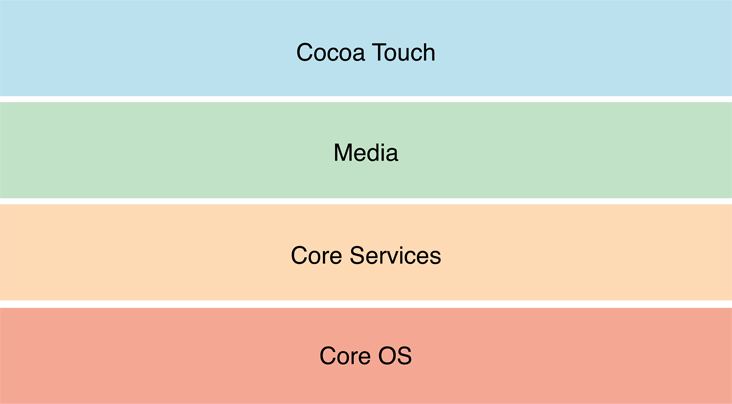
\includegraphics[scale=0.6]{images/iOS_Layers.png}
	\caption{iOS Systemarchitektur (Quelle: \cite[][]{layersOfIos})}
	\label{figIOSSystem}
\end{figure}

Die aus Abbildung \ref{figIOSSystem} ersichtlichen unteren Schichten beinhalten die fundamentalen Dienste. Jede Schicht nutzt die Funktionalitäten der unter ihr liegenden Schicht, um neue anspruchsvollere Dienste zur Verfügung zu stellen.\footcite[vgl.:][]{iOS}\footcite[vlg.:][S. 55 f.]{practicalswift:iosArchitecutre}

Die oberste Schicht, die Cocoa Touch Schicht, bildet mit der von ihr angebotenen Funktionalitäten die Grundlage zur Entwicklung von Applikationen. Bei den hier angebotenen Funktionalitäten handelt es sich um High-Level Features, welche unter anderem App Extensions, Handoff, Document Picker, AirDrop, TextKit, UIKit Dynamics, Multitasking und Auto Layout enthalten.\\
Die Cocoa Touch Schicht bietet somit also die benötigten Funktionalitäten für die Erscheinung sowie der Infrastruktur der Applikation an.\footcite[vgl.:][]{CocoaTouchLayer}

Die zweite Schicht wird als Media Layer bezeichnet und enthält Funktionen für Graphik-, Audio- und Videotechnologien, welche zur Einbindung von Multimediafunktionen in einer Applikation benötigt werden.\footcite[vgl.:][]{MediaLayer}

Auf der dritten Ebene befinden sich die so genannten Core Services.\\
Diese beinhalten fundamentale Systemdienste, welche durch obere Schichten verwendet werden können. Einige dieser Dienste wären beispielsweise Standortsermittlung und Nutzung eines Netzwerks.\\
Diese Dienste werden zum Beispiel für Peer-to-Peer Dienste, die Verwendung des iCloud Speichers sowie SQLite und XML Unterstützung verwendet.\footcite[vgl.:][]{CoreServiceLayer}

Die unterste Schicht bildet das Core OS.\\
Auf dieser Schicht werden low-level Funktionen bereitgestellt, welche für die Verwendung der meisten anderen Technologien benötigt werden.\\
Einige Beispiele wären hier das Bluetooth Framework und das External Accesory Framework, welches es ermöglicht mit Geräten zu kommunizieren, welche an ein iOS-Gerät angeschlossenen sind.\footcite[vgl.:][]{CoreOSLayer}

\subsection{Android}
Android besitzt einen weltweiten Marktanteil von 85\% und wird aktuell von der Open Handset Alliance unter der Leitung von Google weiterentwickelt.\\
Ursprünglich wurde Android von Andy Rubin entwickelt, dessen Unternehmen 2003 von Google aufgekauft wurde.\footcite[vgl.:][]{heiseAndroid}

Nach anfänglichen Startschwierigkeiten hat sich Android heute zum führenden Mobilen Betriebssystem entwickelt. Android wird dabei nicht nur auf Smartphones eingesetzt sondern auch auf Smartwatches, Fernsehern, Tabletts und Autosystemen.\footcite[vgl.:][]{android}

Die rasante Entwicklung von Android und der hohe Gewinn an Marktanteilen ist umso erstaunlicher, betrachtet man das Problem vor dem die Entwickler stehen. Durch die unterschiedlichen Verwendungszwecke von Android und die hohe Anzahl von Geräten unterschiedlicher Hersteller stehen die Entwickler von Android vor der Herausforderung Android stets so zu gestalten, dass es auf selbst ihnen unbekannten Geräten stabil betrieben werden kann.\footcite[vgl.:][]{androidVSios}

\subsubsection{Architektur}
Nachfolgend wird die in Abbildung \ref{figAndroidSystem} sichtbare Architektur von Android näher beschrieben.

\begin{figure}[h]
	\centering
  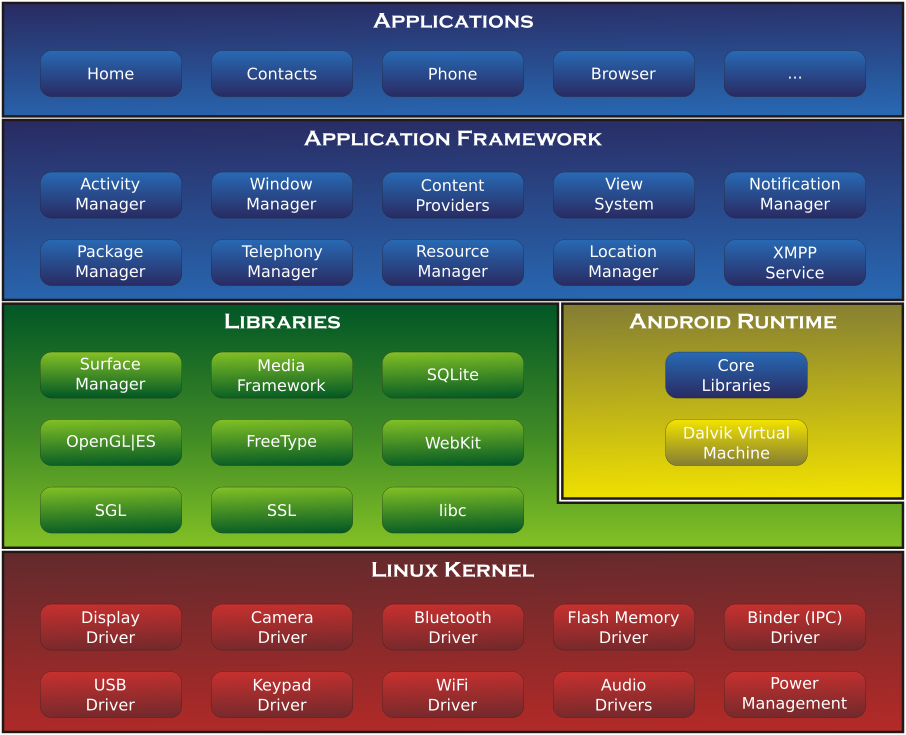
\includegraphics[scale=0.4]{images/Android-System-Architecture.png}
	\caption{Android Systemarchitektur (Quelle: \cite[][]{androidArchitektur})}
	\label{figAndroidSystem}
\end{figure}

Wie aus Abbildung \ref{figAndroidSystem} ersichtlich basiert Android auf einem Linux Kernel. Dieser steuert die Kernfunktionalitäten wie z.B. die Speicher- und Prozessverwaltung als auch das Treibermodell. Der Kernel fungiert somit als Schnittstelle zwischen der restlichen Software und der Hardware des Geräts.\footcite[vgl.:][S. 28 f.]{androidHandbuch}

Die Android Runtime enthält Basisbibliotheken sowie die Dalvik \ac{VM}. Die enthaltenen Basisbibliotheken enthalten die Kernfunktionalitäten der Programmiersprache Java sowie die in C und C++ geschriebenen Komponenten wie beispielsweise OpenGL und OpenSSL.\footcite[vgl.:][S. 9]{einfAndroid} \footcite[vgl.:][S. 27]{androidHandbuch}\footcite[vgl.:][S. 4 f]{braehler:2010}\\
Jede Android Anwendung läuft als eigener Prozess mit eigener Instanz der Dalvik \ac{VM}.\\
Die Dalvik \ac{VM} führt Klassen aus, welche durch einen Java Compiler kompiliert wurden und anschließend in das Dalvik eigene .dex Format, welches besonders speicherschonend ist, transformiert wurden.\footcite[vgl.:][]{androidVSiosArchitekture}\\
Ab Android 5.0 wurde die Dalvik \ac{VM} durch die von Google entwickelte ART Runtime ersetzt. Der Hauptunterschied gegenüber der Dalvik \ac{VM} besteht in der Beschleunigung von Apps und der damit gestiegenen Performance des Systems. Erreicht wird diese Beschleunigung durch eine Ahead-of-Time-Decodierung, bei der Apps bereits bei der Installation übersetzt werden und nicht erst bei der Verwendung wie es bisher unter Verwendung der Dalvik \ac{VM} der Fall war.\footcite[vgl.:][]{artvsdalvik}\footcite[vgl.:][S. 27 f.]{androidHandbuch}

Applikationen für Android werden in Java geschrieben. Android selbst kommt bereits mit einigen Standardapplikationen. Alle von diesen Standardapplikationen verwendeten \ac{API}s die auch für dritte durch das in Graphik \ref{figAndroidSystem} gezeigte Application Framework zur Verfügung gestellt werden. \footcite[vgl.:][S. 10 ff.]{einfAndroid}\footcite[vgl.:][S. 5]{braehler:2010}\\
Die Anwendungsarchitektur ist für eine leichte Wiederverwendbarkeit von Komponenten konizipiert worden. Anwendungen können Komponenten bereitstellen, welche dann wiederum von anderen Anwendungen verwendet werden können.\footcite[vgl.:][]{androidVSiosArchitekture}


\subsection{Vergleich}
Bei der Wahl einer geeigneten Basis für das Projekt \ac{ANNA}, steht vor allem die Erreichbarkeit möglichst vieler Nutzer im Vordergrund.\\
In diesem Punkt liegt Android mit einem Marktanteil von 85\% vor iOS mit einem Marktanteil von 12\%. Die restlichen 3\% teilen sich die weniger verwendeten Betriebssysteme wie beispielsweise Windows Mobile.

Ein weiterer wichtiger Aspekt bei der Wahl des Betriebssystems für \ac{ANNA} besteht im Bereich der Entwicklung des Projekts.\\
Bei der Entwicklung von iOS Applikationen werden die Programmiersprachen Objective-C und Swift verwendet, wohingegen bei der Entwicklung von Android Applikationen die Programmiersprache Java Verwendung findet.\\
Als offizielle Entwicklungsumgebungen werden seitens iOS Xcode verwendet, welches für den Einsatz auf Mac OS konzipiert ist. Für die Entwicklung von Android Applikationen kommt hingegen vorzugsweise die auf IntelliJ basierende Entwicklungsumgebung Android Studio zum Einsatz, die für zahlreiche Betriebssysteme zur Verfügung steht.\\
Beim Entwicklungsprozess spielen auch die durch das Betriebssystem zur Verfügung gestellten Funktionalitäten eine wichtige Rolle.\\
Schränkt das Betriebssystem die Verwendung bestimmter Funktionalitäten zu sehr ein, erschwert dies den Entwicklungsprozess und erfordert mehr Zeit bei der Implementierung geplanter Funktionalitäten des Projekts \ac{ANNA}.

Ein wichtiger Vorteil von iOS gegenüber Android besteht in der nahezu einheitlich verwendeten Betriebssystemversion.\\
Durch die Selbstverantwortlichkeit von Apple für die Verteilung neuer Softwareversionen, besteht hier der Vorteil, dass stets die neuste Betriebssystemversion auf allen unterstützten Geräten installiert wird.\\
Bei Android hingegen sind die einzelnen Gerätehersteller dafür verantwortlich die neuste von Google bereitgestellte Version auf ihren Geräten zu verteilen. Durch diesen Umstand sind eine Vielzahl unterschiedlicher Android Versionen im Einsatz, welche sich auch in ihrem Funktionsumfang unterscheiden. Diese Unterschiede führen bei der Entwicklung dazu, dass nicht alle Android Versionen unterstützt werden können und man so einen Prozentualen Teil der potentiellen Nutzer ausschließen muss.\footcite[vgl.:][]{androidvsiosvergleich}

Um den Entwicklungsprozess durch das Erlernen einer neuen Programmiersprache nicht weiter hinauszuzögern und das Entstehen zusätzlicher Kosten durch fehlende Apple Testgeräte zu vermeiden, fällt die Wahl des Betriebssystems bei diesen Kriterien auf Android.\\
Auch durch die größere Anzahl potentieller Nutzer sowie den große Freiraum bei der Entwicklung, fiel auch bei diesem Kriterium die Wahl auf Android.\\
Trotz der großen Fragmentierung durch die Verbreitung unterschiedlicher Android Versionen, welche unter iOS nicht vorhanden ist, überwiegen die positiven Ergebnisse bei den restlichen Kriterien, so dass als Basis für Projekt \ac{ANNA} das Betriebssystem Android zum Einsatz kommt.

Tabelle \ref{tabAndroidVsIOS} bietet nochmals eine übersichtliche Darstellung der einzelnen Ergebnisse des Vergleichs.
\begin{table}[h]
\centering
\begin{tabular}{ |c|c|c| } 
 \hline
 & iOS & Android \\
 \hline
 Entwicklungssprache & Objective-C/Swift & Java \\
 Entwicklungsumgebung & Xcode & Android Studio  \\
 Zugriff & Limitiert & Nahezu Restriktionsfrei   \\
 Marktanteil &12\% & 85\%\\
 Fragmentierung & gering & hoch\\
 \hline
\end{tabular}
\caption{Vergleich iOS und Android}
\label{tabAndroidVsIOS}
\end{table}

%-beide haben Sicherheitslücken, allerdings werden diese schnell geschlossen

\section{Mikrofon}
\label{chpt:Mic}
In dieser Sektion wird speziell auf die verschiedenen Konfigurationsmöglichkeiten des eingebauten Mikrofons und externer Mikrofone eingegangen, da diese eine gravierende Auswirkung auf die Qualität der Spracheingabe mit sich bringen. Dabei spielen insbesondere die beiden Punkte Position und Design eine große Rolle.

\subsection{Position}
Die Abhängigkeit der Erkennungsrate im Hinblick auf die Position des Smartphones wird besonders deutlich, wenn die Lautstärke im Innenraum des PKW betrachtet wird.
In der Tabelle \ref{tabLautMessungFahrt} sind die Messergebnisse einer Innenraum Schallmessung eines PKW im Straßenverkehr festgehalten.%TODO Fußnote Verwendete App
Dabei ist die durchschnittliche Lautstärke abhängig von der Fahrbahn, dem Wetterverhältnis und der Radioeinstellung. 

Bei einem durchschnittlichen Messwert von 56 dB, welcher im Stand bei laufendem Motor gemessen wurde, ist die Position im Auto nicht ausschlaggebend. Dies bedeutet unabhängig von der Position wurde eine Erkennungsrate von über 90 Prozent erzielt, wobei direkt am Mund die höchste Prozentzahl erreicht wurde. Unter Betrachtung einer durchschnittliche Lautstärke von 80 dB auf der Autobahn resultiert ein deutlicher Einfluss der Sprachqualität. Dies folgt daher, da die Dezibel Skala nicht linear sondern logarithmisch ist. Der Unterschied zwischen einem stehenden Auto (56 dB) und einem fahrenden (80 dB) liegt daher bei dem Faktor 4, welches daraus resultiert, dass 6 dB bereits eine Verdopplung der Lautstärke bewirken. 

Aufgrund dieser Differenz folgt eine große Menge an Störgeräuschen, welche von der Speech APi, \ac{CMU}, herausgefiltert werden müssen, um die Eingaben des Nutzers zu erkennen. Dafür wird im Hinblick auf \ac{CMU} der Spektrale Substraktions Algorithmus verwendet. Unter Verwendung dieses Algorithmus wird trotz erhöhter Umgebungslautstärke eine annehmbare Erkennungsrate erreicht. Zusammen mit der Position kann diese Erkennungsrate sowohl verbessert als auch verschlechtert werden. 

Die verschiedenen Positionen, welche in Bild \ref{figMikroPositionen} zu sehen sind, kombiniert mit unterschiedlichen Smartphones repräsentieren die Erkennungsraten, die in Tabelle \ref{tabErkennungsrate} stehen. Dabei kristallisiert sich heraus, dass die intern verbauten Mikrofone starke Abweichung je nach Smartphone Modell haben. So weist das Mikrofon vom Nexus 5X eine 50 Prozent bessere Erkennungsrate als das LG G2 auf. Gründe für diesen drastischen Unterschied sind das verbaute Mikrofon und die Betriebssystemversion des Smartphones. Zusätzlich lässt sich erkennen, dass zwei der drei Positionen des Smartphones sich von der Erkennungsrate her kaum unterscheiden, jedoch die Position Mittelkonsole eine deutliche Verschlechterung aufweist.
%Lässt sich durch die Grundlegende Wellen Physik beweisen -> Verschlechterung der Qualität. Listing mit Formel Wellenausbreitung in einer Richtung
Dies lässt sich darauf zurückführen, dass die Sprechrichtung des Nutzers nach vorne hin zur Straße gerichtet ist und somit nur eine deutlich verminderte Qualität des gesprochenen in der Mittelkonsole ankommt.

Somit sollte sich das Mikrofon und damit auch das Smartphone unmittelbar vor dem Fahrer des Fahrzeugs oder in einer Halterung in der Nähe des Lenkrads befinden, um eine ideale Qualität der Spracheingaben zu gewährleisten. Zusätzlich empfiehlt sich bei älteren Handy Modellen die Verwendung externe Mikrofone, welches in Sektion \ref{sctAddMic} genauer beschrieben ist. 

\begin{figure}[h]
	\centering
  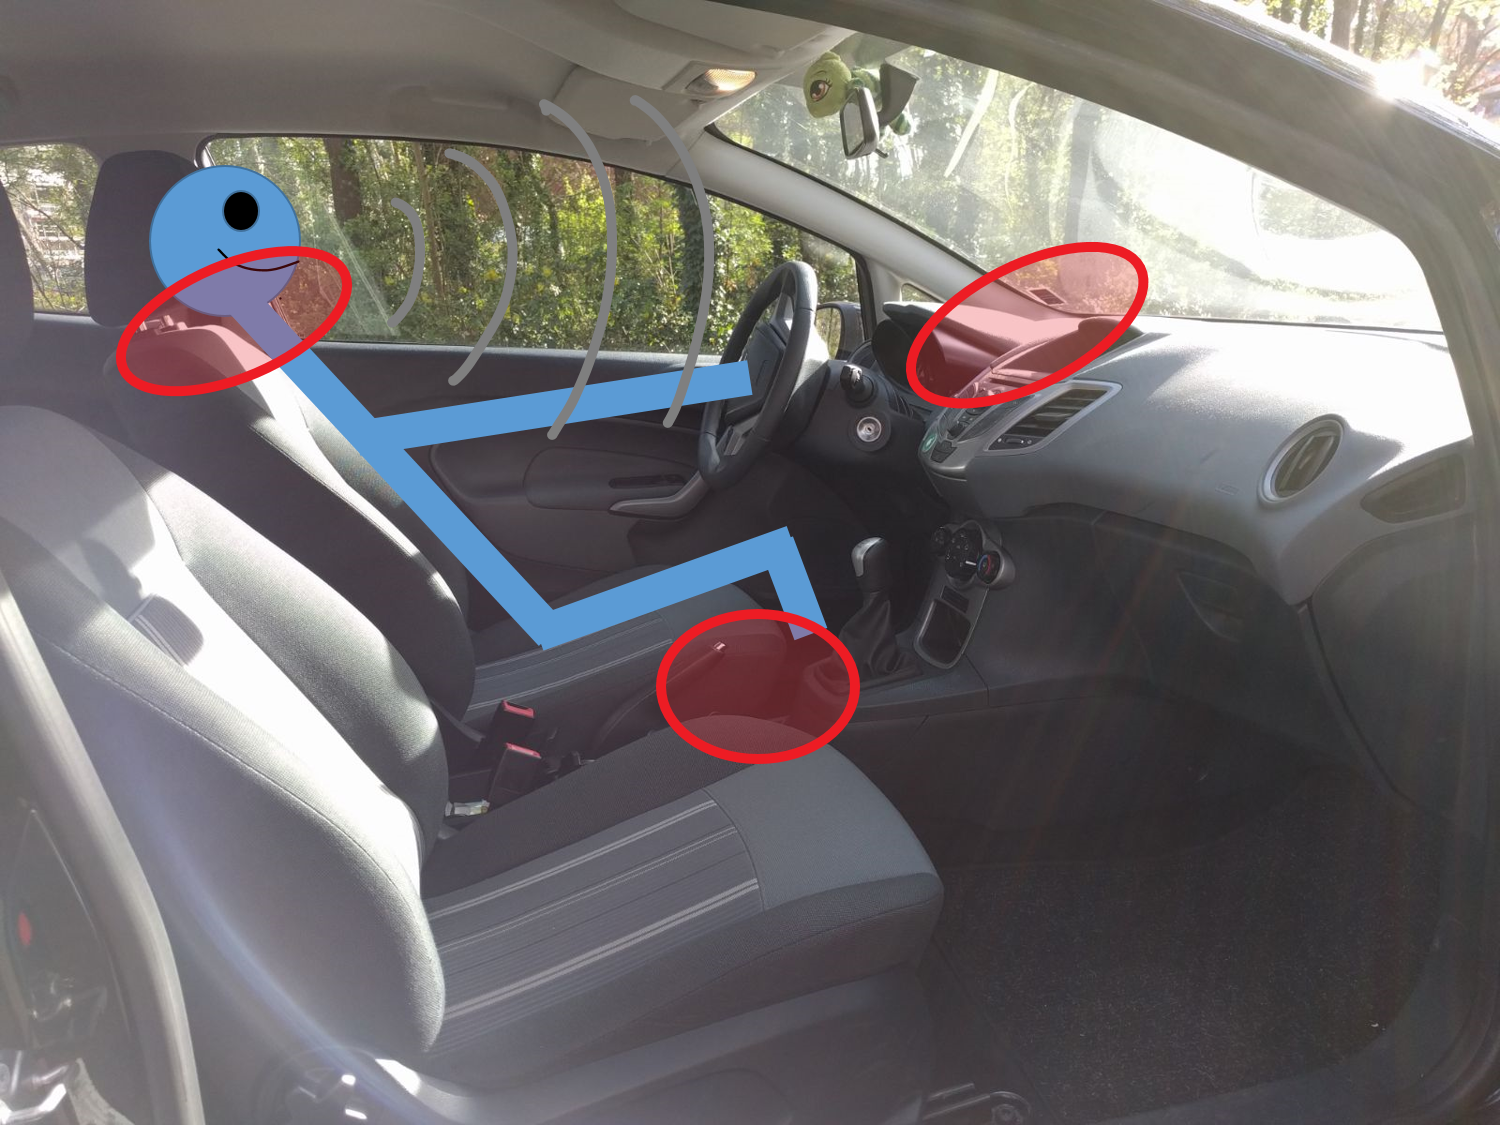
\includegraphics[scale=0.3]{images/position_waves.png}
	\caption{Ford Fiesta Mikrofon Positionen}
	\label{figMikroPositionen}
\end{figure}

\begin{table}[h]
\centering
\begin{tabular}{ |c|c|c|c| } 
 \hline
 Fahrbahn & Wetter & Radioeinstellung & Lautstärkedurchschnitt\\
 \hline
 Autobahn & Regen & Laut & 90dB\\
 Autobahn & Regen & Mittel & 82dB\\
 Autobahn & Regen & Leise & 80dB\\
 Autobahn & Bewölkt & Leise & 77dB\\
 Landstraße & Regen & Laut & 90dB\\
 Landstraße & Regen & Mittel & 81dB\\
 Landstraße & Regen & Leise & 77dB\\
 Landstraße & Bewölkt & Leise & 75dB\\
 Stadt & Bewölkt & Leise & 72dB\\
 \hline
\end{tabular}
\caption{Lautstärkemessung in einem Ford Fiesta Baujahr 2009 }
\label{tabLautMessungFahrt}
\end{table}

\begin{table}[h]
\centering
\begin{tabular}{ |c|c|c|c|c| } 
 \hline
 Smartphone & Mikro & Position & Erkennungsrate & OS Version\\
 \hline
 Nexus 5X & Intern & Am Mund & 95\% & Android 7.1\\
 Nexus 5X & Intern & In Halterung & 90\% & Android 7.1\\
 Nexus 5X & Intern & Mittelkonsole & <10\% & Android 7.1\\
 Nexus 5X & Teufel Move & Am Hals & 98\% & Android 7.1\\
 Nexus 5X & No Name Headset & Am Hals & 88\% & Android 7.1\\

 Samsung S3 & Intern & Am Mund & 92\% & Android 6.1\\
 Samsung S3 & Intern & In Halterung & 88\% & Android 6.1\\
 Samsung S3 & Intern & Mittelkonsole & <5\% & Android 6.1\\
 Samsung S3 & Teufel Move & Am Hals & 95\% & Android 6.1\\
 Samsung S3 & No Name Headset & Am Hals & 85\% & Android 6.1\\

 LG G2 & Intern & Am Mund & 85\% & Android 5.1\\
 LG G2 & Intern & In Halterung & 40\% & Android 5.1\\
 LG G2 & Intern & Mittelkonsole & <5\% & Android 5.1\\
 LG G2 & Teufel Move & Am Hals & 90\% & Android 5.1\\
 LG G2 & No Name Headset & Am Hals & 85\% & Android 5.1\\

 \hline
\end{tabular}
\caption{Erkennungsrate von \ac{ANNA} Sprachbefehlen}
\label{tabErkennungsrate}
\end{table}

\subsection{Design}
%Elektret-Kondensatormikrofone Funktionsweise mit Darstellung
In nahezu allen modernen Konsumergeräte, welche ein Mikrofon verbaut haben, wird das Elektret-Kondensatornmikrofon, auch dauerpolarisierte Kondensatormikrofone genannt, verbaut.
Dieses Mikrofon zeichnet sich durch zahlreiche Vorteile gegenüber anderen Mikrofonarten aus.
\footcite[vlg.:][]{micNutzung}

Die Vorteile resultieren aus dem Aufbau des Mikrofons, welche in Grafik \ref{figElektretMic} zu sehen sind Gegenüber dem normalen Kondensatormikrofon, verwendet das Elektret-Mikrofon als Membran anstatt eines Kondensators eine dauerhaft polarisierte Elektretfolie, wodurch nur der anschließende Feldeffekttransistor zur Verstärkung des Signals mit 1,5 Volt betrieben werden muss. Wohingegen das Kondensator Mikrofon eine dauerhafte Phantomspeisung von 48 Volt benötigt. Aufgrund dieser niedrigen Betriebssppannung, der Kompaktheit und den Herstellungskosten ist das Elektret-Mikrofon in derart vielen Endgeräten verbaut.
\footcite[vlg.:][S. 45 f.]{microphoneBook}

Im Prozess der Tonaufnahme dient das Elektret-Mikrofon als Schallwandler, da es die einfallenden Schallwellen in elektrische Spannungsänderungen transformiert. Die auf die Membran der Elektretkapsel auftreffenden Schallwellen bringen diese zum Schwingen. Die Umwandlung der Schallwellen in elektrisch auswertbare Signale erfolgt durch die Kapazitätsänderung in der Elektretkapsel. Diese lässt sich zeitaufgelöst messen und wird damit zum digitalsierten Abbild der eintreffenden Schallwellen.
\footcite[vlg.:][S. 45 f.]{microphoneBook}\footcite[vlg.:][]{funktionsweiseMic}

\begin{figure}[h]
	\centering
  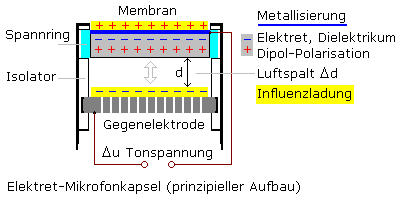
\includegraphics[scale=0.75]{images/aufbau_mic.png}
	\caption{Prinzipieller Aufbau eines Elektret-Mikrofons (Quelle: \cite[][]{funktionsweiseMic})}
	\label{figElektretMic}
\end{figure}


\subsection{Zusätzliches Mikrofon}
\label{sctAddMic}
Aufgrund lauter Umgebungsgeräusche, während der Führung eines Kraftfahrzeuges, fällt die Erkennungsrate je nach Smartphone drastisch ab, welches in Tabelle \ref{tabErkennungsrate} zu sehen ist. Um diesen Fall entgegen zu wirken, empfiehlt sich die Verwendung eines externen Mikrofons. 

Ein externes Mikrofon ist dazu in der Lage, abhängig von seiner Position, die Sprachqualität und somit auch die Erkennungsrate erheblich zu steigern. Als externe können Inear-Headsets, Bluetooth-Headsets aber auch die Freisprecheinrichtung des Autos verwendet werden. Im Rahmen von Testfahrten wurden insbesondere Inear-Headsets getestet. Die Ergebnisse dieser Testfahrten sind in Tabelle \ref{tabErkennungsrate} festgehalten.

Wie der Tabelle zu entnehmen ist wurde sowohl ein Markenheadset, Teufel Move, als auch ein No Name Headset getestet. Unabhängig von der Qualität des Headsets wurde allein durch die Verwendung eines externen Mikrofons eine deutliche Steigerung der Erkennungsrate erreicht, welches sich auf den Abstand zum Mund und die Qualität des Mikrofons zurückführen lässt. Zum Beispiel wurde so eine Steigerung von knapp 50 Prozent in einzelnen Fällen erreicht.

Bei genauerer Betrachtung der beiden Headsets wird lediglich eine minimale Erhöhung der Erkennungsrate deutlich. Auch spielt der Wahl des Smartphones im genaueren des Betriebssystems eine Rolle, da aufgrund des dominierenden Marktanteils von Android, eine deutlich größere Zahl externe Mikrofone zur Verfügung steht.

\subsection{Ergebnis}
Es gibt viele Einflussfaktoren, welche die Sprachqualität und Erkennungsrate der Applikation sowohl positiv als auch negativ beeinflussen können. Die Wichtigsten sind: Position, Typ und Qualität des Mikrofons. Aus unseren Analysen, Testfahrten und physikalischen Grundlagen resultiert die optimale Position des Mikrofones in Höhe der Sprachquelle. Echte Kondensatormikrofone könnten die Erkennungrate weiter verbessern. Wegen des hohen Preises dieser technisch anspruchsvollen Mikrofonvariante scheidet diese für den Masseneinsatz aus.
Abschließend lässt sich feststellen: aktuelle Smartphones liefern wegen der bereits verbauten hochwertigen Komponenten bei guter Positionierung annehmbare Erkennungsraten.  
Bei älteren Smartphones lässt sich die Erkennungsrate bei Einsatz externer Mikrofen auf ein annehmbares Niveau steigern.


\section{Vergleich bestehender Applikationen}
Im Rahmen dieser Sektion wird das Projekt einschließlich der Anforderungen und Ziele mit bestehenden Applikationen verglichen, welche ähnliche Ideen verfolgen. Hinsichtlich dieses Vergleiches wurden die Applikationen Automate-Armaturenbrett und Android Auto ausgewählt. Automate aufgrund der hohen Nutzergruppe und Android Auto, da die Applikation direkt an verschiedenste Google Diensten, beispielsweise Maps oder Hangouts angebunden ist. 
\subsection{Automate}
Automate verfolgt die Idee eines Dashboards für das Auto, damit der Fokus im Auto wieder auf die Straße gelenkt wird. Um dieser Idee gerecht zu werden, sind zahlreiche Funktionen in die Applikation integriert. Dazu zählen das reagieren auf eingehende Nachrichten, das Anrufen von Telefonkontakten, die Navigation von Startpunkt A nach Endpunkt B und die Einbindung des Musikdienstes Spotify und der auf dem Smartphone vorliegenden Musik.
Die integrierten Funktionen spiegeln sich im Layout der Applikation wieder wie in Abbildung \ref{figAutomate} zu sehen ist. Im unteren Teil der Applikation befindet sich verschiedene Icons, welche auf die jeweilige View verweisen. Des Weiteren gibt es eine Overall View, welche in der Abbildung zu sehen ist. Auf dieser View sind wichtige Informationen auf einem Blick zu sehen.
\begin{figure}[h]
	\centering
  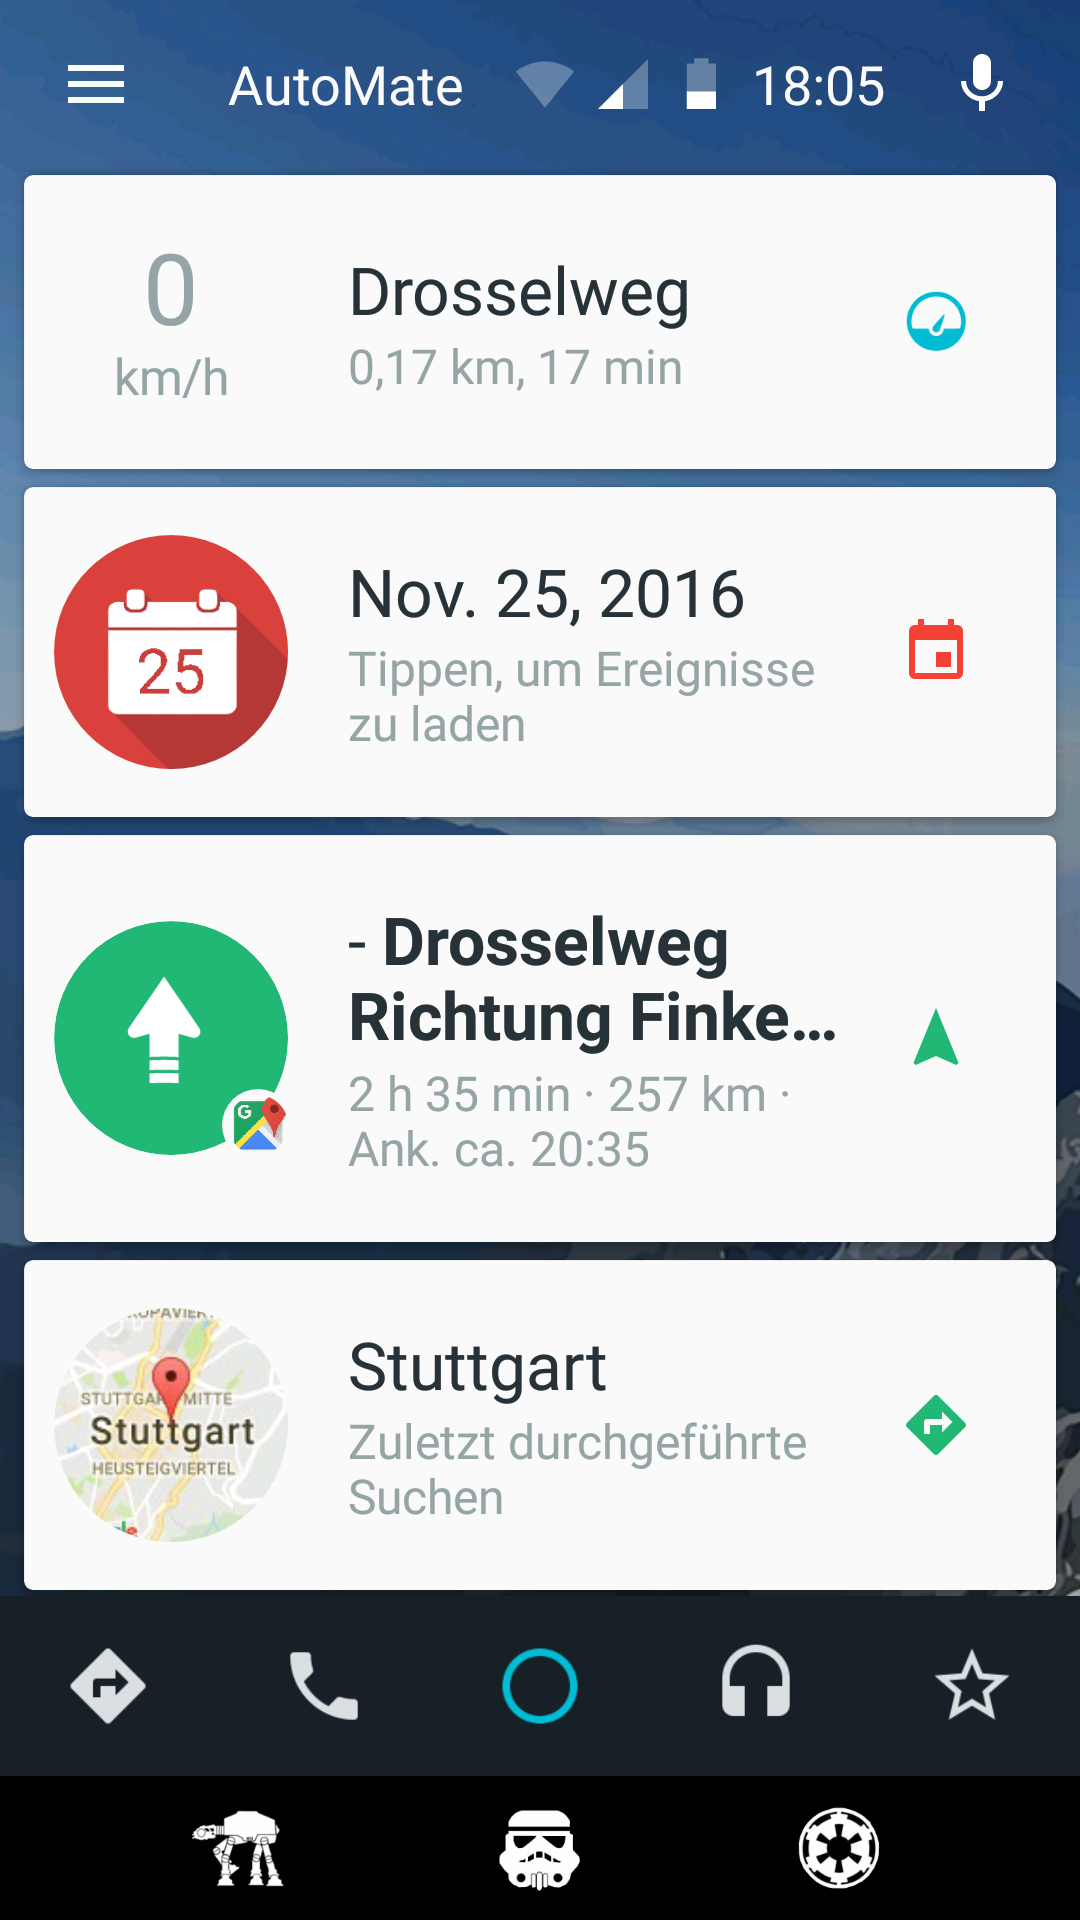
\includegraphics[scale=0.2]{images/Automate_Dashboard.png}
	\caption{Automate Screenshot}
	\label{figAutomate}
\end{figure}
Vergleichbare Strukturen sind auch in den Anforderungen und Zielen dieser Arbeit zu finden. Jedoch wird in Automate eine Modulare Selektierung nicht angeboten. Dies bedeutet, dass dem Benutzer immer alle Funktionalitäten zur Verfügung stehen, auch diese die nicht im Interesse des Benutzers liegen. Im Hinblick auf das Ziel der Applikation, den Fokus auf die Straße zu legen, wird eine Schlüsselwort basierte Aktivierung der Spracherkennung nicht angeboten. Somit ist der Benutzer der Applikation gezwungen, das Mikrofon bei gewünschter Eingabe über einen Knopfdruck zu aktivieren. Die Schlüsselwort Erkennung ist wie in Kapitel \ref{sec:requirements} angesprochen ein Anforderung an das Projekt und in der finalen Applikation enthalten, um eine komplett berührungslose Interaktion nach dem Starten zu schaffen. 

Sowohl Automate als auch \ac{ANNA} sind in der Lage eingehende Nachrichten vorzulesen und auf diese zu antworten. Dies funktioniert bei beiden mit einer Vielzahl von modernen Messengern wie Whats App, Hangouts und Telegram. Allerdings unterscheiden sich die Applikationen in der Spracherkennung. Automate als Sprachinterface Google Now, welches standardmäßig Nachrichten verschicken oder Anrufe tätigen kann. Die Benutzung dieses Interfaces zieht jedoch einen hohen Datenvolumen Verbrauch mit sich, da die Worterkennung auf den Google Servern absolviert wird. Um Ressourcen zu schonen wird bei \ac{ANNA} eine offline fähige Speech \ac{API} namens ,,Voice Action'' benutzt. Dadurch können Sprachkommandos direkt auf dem Smartphone gerechnet werden. 

Eines der Ziele eines Auto Dashboards ist die Navigation, weshalb Automate als auch \ac{ANNA} die Benutzung von Navigationsoftware anbieten. Beispielsweise integrieren beide Applikationen Google Maps als Navigationsservice. Dennoch unterscheiden sich die beiden in der Integrierung des Services. Bei Automate wird beim Eingeben eines Zielortes Google Maps als eigene Applikation gestartet und danach in eine View von Automate geladen. Da Google Maps nicht komplett als eigenständiger Service eingebunden wird, geht sowohl Funktionalität als auch Performance verloren. Im Gegensatz dazu ist Google Maps als eigener Service in \ac{ANNA} eingebaut, wodurch ein kompletter Zugriff auf Funktionalitäten und Performance gewährleistet ist.

Zusammenfassend lässt sich sagen, dass beide Applikationen ihres Zieles gerecht werden, aber sich in ihrer Umsetzung unterscheiden.

\subsection{Android Auto}
Mit Android Auto bietet Google ihren eigenen Auto-Dashboard Applikation an, welche den Google Now Sprachdienst als Basis benutzt. Durch diese Applikation wird der Fokus vom Handy wieder auf die Straße gelenkt, da auch hier die Idee der berührungslosen Interaktion verfolgt wird.
Um diese Idee umzusetzen integriert Android Auto eine Vielzahl an verschiedenen Applikationen, welche über Sprachbefehle gesteuert werden können. Diese decken verschiedene Funktionalitäten wie Navigation, Musik-Streaming und Kommunikation ab, wobei diese Apps größtenteils von Google stammen, zum Beispiel Google Maps, Google Music oder Google Hangouts. Allerdings sind auch externe Kommunikations- sowie Musikdienste, wie beispielsweise WhatsApp, Telegram oder Spotify, eingebunden. 
Dabei spiegelt das User Interface diese Funktionalitäten in mehreren Screens wieder. In Grafik \ref{figAndroidAuto} ist der Aufbau und Verweis auf diese Screens zu sehen, welche sich in einen Home-, Navigation-, Telefon- und Musikscreen unterteilen. Ähnlich wie bei Automate stehen dem Nutzer jederzeit alle Funktionalitäten zur Verfügung, allerdings auch die, die er nicht benötigt.      
\begin{figure}[h]
	\centering
  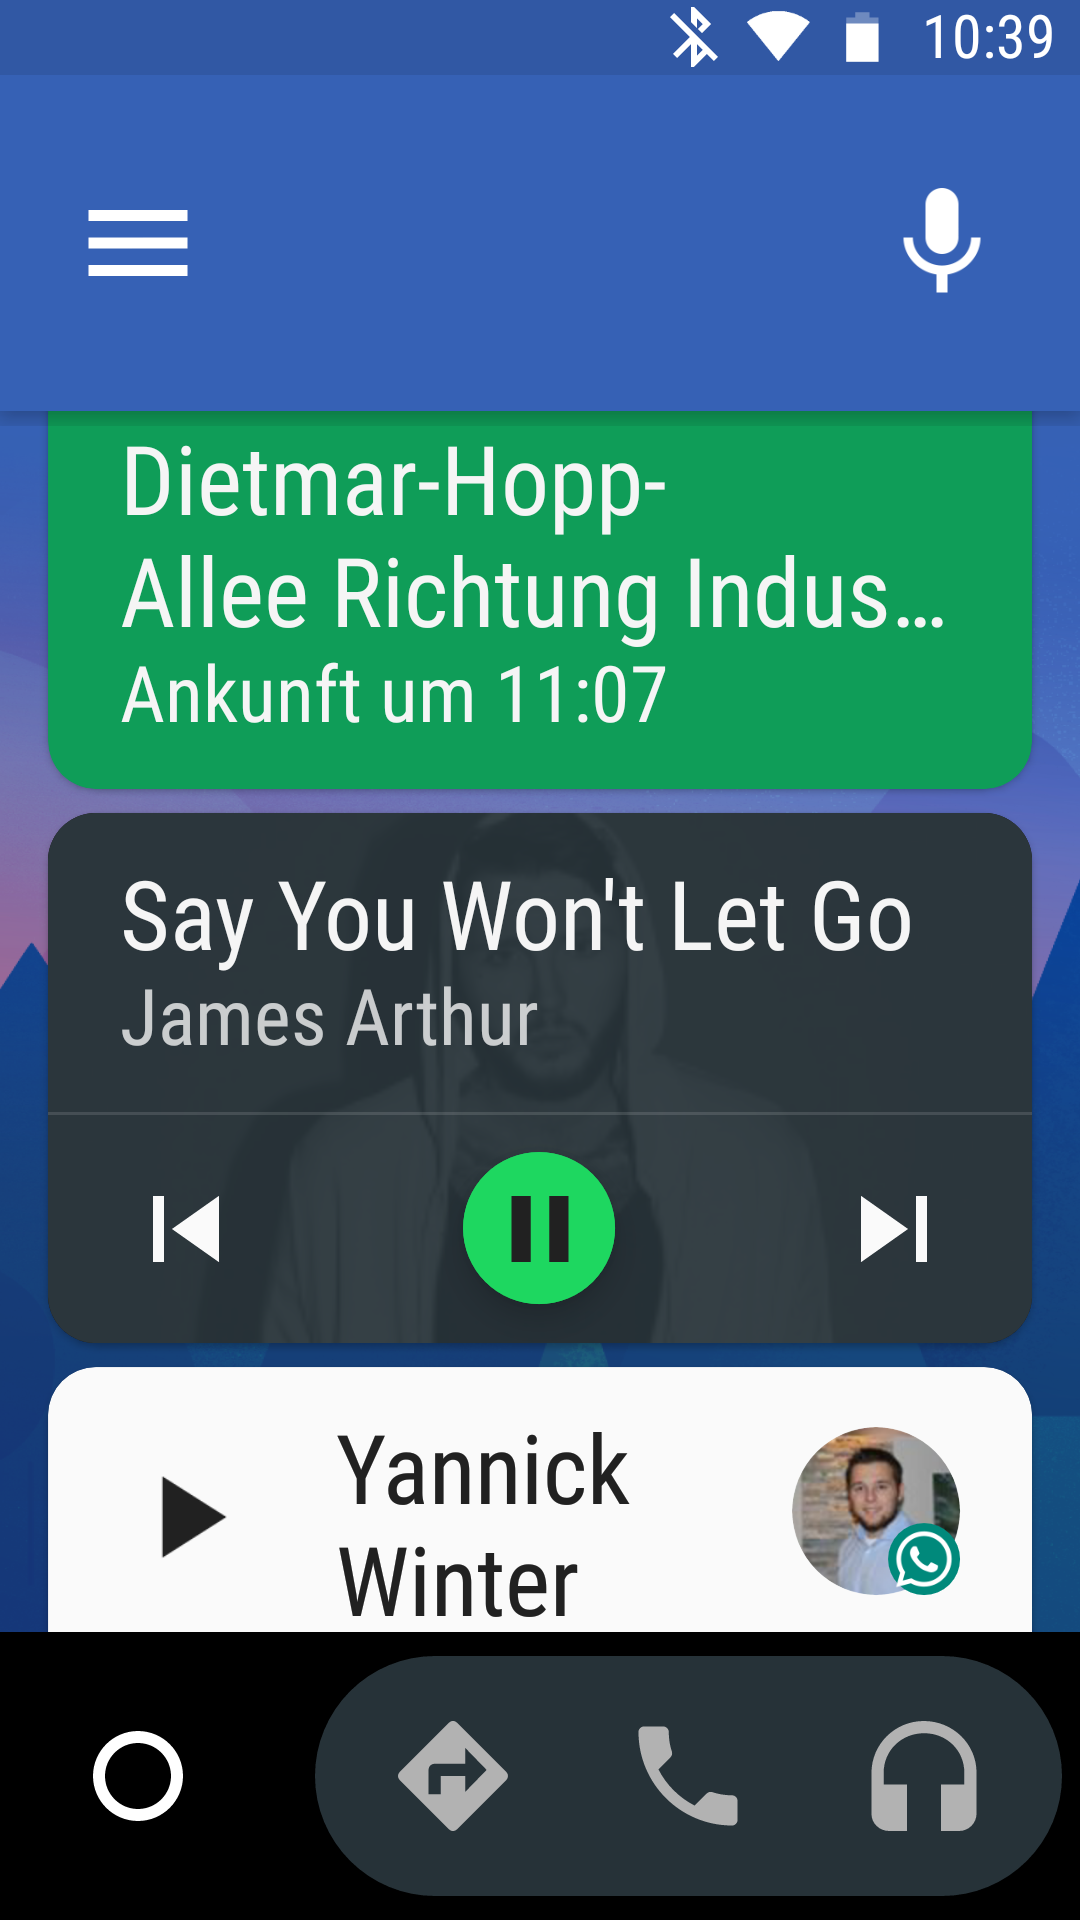
\includegraphics[scale=0.18]{images/Android_Auto.png}
	\caption{Android Auto Screenshot}
	\label{figAndroidAuto}
\end{figure}
Im Hinblick auf die Navigation ist Google strikt und erlaubt als einzigen Dienst das Firmen eigene Google Maps. \ac{ANNA} bietet hier zusätzlich andere Services wie beispielsweise Here Maps.

Android Auto verfolgt als Dashboard Applikation das Ziel der berührungslosen Interaktion, welches mit der Hot Word Erkennung von Google Now im Fundament erreicht wird, bietet jedoch keine weitreichende Steuerung über Spracheingaben an. Befehle, die von Google Now bereits beherrscht werden gezielt umgesetzt. Dies sind zum Beispiel das Versenden von Nachrichten als SMS oder WhatsApp, das Starten einer Navigation oder Anzeigen von Points of Interests auf der Route und das Anrufen von Kontakten. Allerdings erfordern viele weitere, von Android Auto bereitgestellte, Funktionalitäten das Bedienen des Smartphones mit der Hand. Dazu zählen das direkte Antworten auf eingehende Nachrichten und das Steuern von der Musik Dienste. Da diese Funktionalitäten jeder oft genutzt werden und zugleich Kernfunktionen der Applikation darstellen, erzeugen sie wiederum Ablenkungen für den Fahrer, welches dem Gedanken hinter diesem Produkt widerspricht. Im Gegenteil dazu ist es das Ziel im Projekt \ac{ANNA} eine vollständige Kommunikation zwischen Fahrer und Software über Spracheingaben zu schaffen. Wodurch das Fahren des Verkehrsmittels klar im Vordergrund steht. 

Spracheingaben können je nach Konfiguration des Google Dienstes entweder online mit Hilfe von Servern oder offline direkt auf dem Smartphone analysiert und berechnet werden. Wird danach ein Internetzugriff benötigt schickt Google die zuvor berechnete Spracheingabe an die benötigte Applikation oder Service. In diesem Punkt ähneln sich sowohl Android Auto als auch \ac{ANNA}, um in Punkto Zuverlässigkeit den Nutzer zufrieden zu stellen. 

Aus Performance technischer Sicht steht Android Auto gut dar. Dies ist auf die Anbindungsweise der einzelnen Services zurückzuführen. Aufgrund der Tatsache, dass Google die meisten integrierten Services selbst entwickelt hat, kann ein einfacher und schneller Zugriff erfolgen. \ac{ANNA} hingegen benutzt entweder selbst entwickelte oder frei verfügbare \ac{API}s, welche nicht immer vom Entwickler der Services bereitgestellt wurden. Daraus lässt sich meist eine längere Ab- und Anfragezeit ableiten.

Abschließend lässt sich sagen das Android Auto zurzeit relativ wenig Funktionalität anbietet, diese jedoch großenteils gut umsetzt. Jedoch bieten Sprachkontrolle der Applikation und das Einbinden externer Services noch Optimierungspotential.

	\chapter{Implementierung}

\section{Use Cases}
Graphik \ref{figUseCaseDiagram} bietet einen anschaulichen Überblick über die definierten Use Cases und durch welche Funktionalitäten sie sich zusammensetzen.

\begin{figure}[h]
	\hspace*{-1.5cm}
  \includegraphics[scale=0.5]{images/Use_Case_Diagram.png}
	\caption{Use Case Diagram}
	\label{figUseCaseDiagram}
\end{figure}

Der eigentliche Use Case des Systems besteht in der berührungslosen Interaktion mit dem Smartphone.\\
Um diesen Use Case umzusetzen, ist die Interaktion mit verschiedenen Bereichen des Smartphones erforderlich, welche mit Hilfe der Funktionalitäten aus der Kategorie Voice Recognition gesteuert werden können.

Die Funktionalitäten aus der Gruppe der Voice Recognition Use Cases, beinhaltet die Use Cases für die primäre Kommunikationsschnittstelle zwischen Nutzer und System. Diese Gruppe enthält die Use Cases die vom Nutzer direkt verwendet werden können. Durch die Verwendung dieser Funktionen wird es dem Nutzer ermöglicht auf die restlichen Funktionalitäten zuzugreifen.\\
Die Use Cases dieser Kategorie umfassen eine Hotword Detection, welche in Sektion \ref{scthotword} näher beschrieben wird, die Speech-to-Text Umwandlung, welche für die generelle Verwendung der Spracheingabe benötigt wird, sowie die darauf basierende Menüführung, welche der Interaktion mit anderen Bereichen des Smartphones dient.\\
Bei der Entwicklung dieser Funktionen liegt ein hoher Stellenwert auf dem Datenschutz der Nutzer. Die Sprachaufnahmen werden nur so lange genutzt wie es wirklich notwendig ist. Ist die Umwandlung und damit die Auswertung der Sprachaufnahme abgeschlossen, wird sie umgehend gelöscht.

Einer der bereits erwähnten Bereiche beinhaltet die auf dem Smartphone installierten Messenger. 
Durch die Integration der meistverwendeten Messenger des jeweiligen Nutzers, ist es dem Nutzer möglich, alle eingehenden Nachrichten sofern er es wünscht wahrzunehmen und auch direkt auf diese zu antworten. Mit Hilfe der Spracherkennungsfunktionalitäten, wird es dem Nutzer ermöglicht, auf eingehende Nachrichten zu reagieren, ohne den Blick von der Fahrbahn abwenden zu müssen.\\
Eine weitere große Gruppe besteht in der Kategorie der Musik-Applikationen. Durch die Verwendung der bereits erwähnten Spracherkennungsfunktionen, wird es dem Nutzer ermöglicht sich durch Lieder zu navigieren ohne seine Hände vom Lenkrad nehmen zu müssen. Die Funktionalitäten die dem Nutzer somit zur Verfügung gestellt werden sind das Abspielen und Stoppen von Musik sowie Lieder zu überspringen.\\
Die dritte größere Gruppe von Use Cases stellt die Navigationsintegration dar. Die Applikation \ac{ANNA} liefert dem Nutzer eine bereits komplett integriertes Navigationssystem, welches es dem Nutzer ermöglicht Routen zu berechnen sowie sich mit Hilfe einer Turn-by-Turn Navigation zum gewünschten Ziel führen zu lassen. Die Funktionen dieser Gruppe lassen sich vom Nutzer sowohl direkt ausführen, beispielsweise wenn der Nutzer vor Fahrtbeginn den Navigationsmodus starten möchte, als auch über die Funktionalitäten der Spracherkennung, falls der Nutzer möglicherweise bereits im Straßenverkehr unterwegs ist und merkt, dass er sich nicht sicher ist welche Route er am besten nehmen soll um an sein gewünschtes Ziel zu kommen.

Um dem Nutzer die Verwendung seines Smartphones so angenehm wie möglich zu gestalten, ist ebenfalls die Anruf Funktionalität in die Applikation \ac{ANNA} integriert. Der Nutzer hat somit die Möglichkeit sowohl Kontakte in seinem Telefonbuch anzurufen, als auch fremde Nummern anzurufen.\\
Ein weiterer wichtiger Punkt zur Verbesserung der Nutzer Erfahrung, ist die Regulierung der Bildschirmhelligkeit abhängig vom Lichteinfall. Um den Nutzer während der Fahrt bei schlechten Lichtverhältnissen nicht zu blenden, wird die Helligkeit des Displays herab gesenkt, indem für die Benutzeroberfläche verwendete Farben zu dunkleren Tönen verändert werden.

Unter dem Reiter Einstellungen, ist es dem Nutzer möglich seine bei der Initialisierung der App ausgewählten Module zu ändern. So kann der Nutzer stets die Anwendung an seine Bedürfnisse anpassen falls diese sich ändern sollten.\\
Die Use Cases dieser Kategorie stellen die einzigen Funktionen dar, welche direkt vom Nutzer verwendetet werden können, ohne dass zunächst eine Funktionalität aus der Gruppe der Spracherkennung verwendet wird. Der Grund für diese direkte Nutzung liegt darin, dass diese Gruppe der Use Cases keine Funktionalitäten enthält die während der Fahrt benötigt werden könnten.

\section{Architektur der Applikation}
Nachfolgend wird die in Abbildung \ref{figClassDiagram} dargestellte Architektur der Applikation \ac{ANNA} erläutert.\\
Der Aufbau der Applikation entspricht aufgrund der Struktur des Android Betriebssystems der \ac{MVC} Architektur.

\begin{figure}[h]
\hspace*{-2.2cm}
  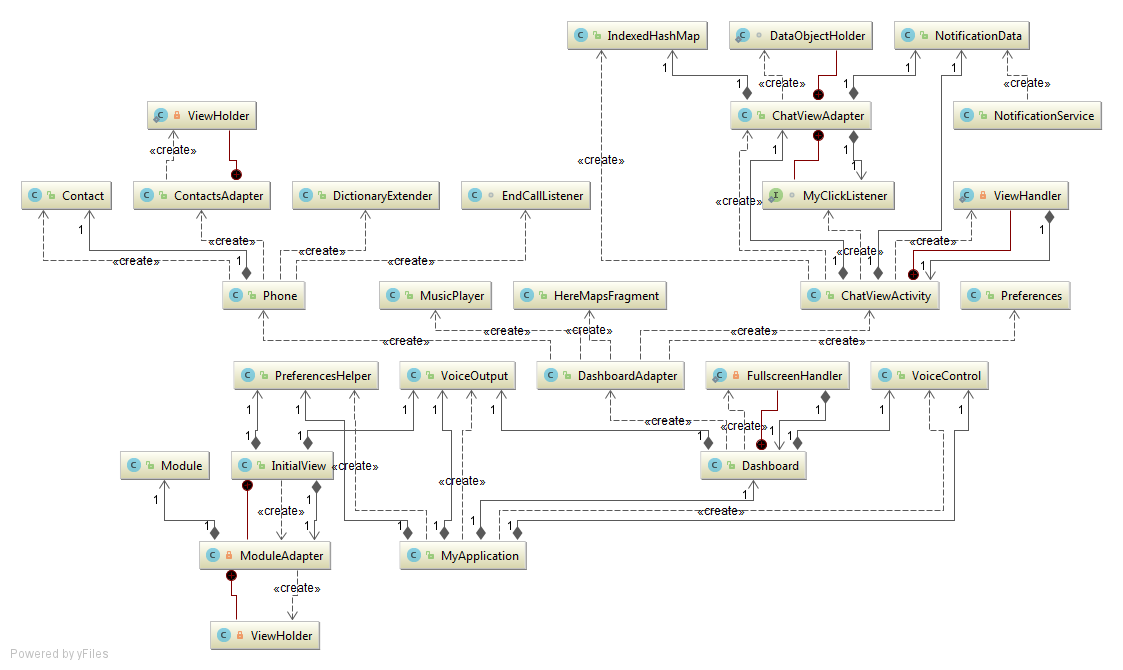
\includegraphics[scale=0.5]{images/diagram.png}
	\caption{Klassen Diagramm}
	\label{figClassDiagram}
\end{figure}

Die Klasse MyApplication dient repräsentativ für die Applikation \ac{ANNA}. Es gibt nur eine Instanz dieser Klasse und entspricht somit dem Programmierparadigma Singleton.\\
Durch den Start der Anwendung, wird durch das Android Betriebssystem eine Objekt dieser Klasse initialisiert. Anschließend werden Instanzen aller Klassen erstellt, welche häufig von anderen Objekten verwendet werden. Über den Aufruf der Instanz von MyApplication, ist es somit anderen Objekten möglich auf Funktionalitäten wie Sprachausgabe, Sprachsteuerung und den Applikationskontext zuzugreifen.\\
Die Klasse MyApplication dient somit als zentrale Schnittstelle für den internen Zugriff der bereitgestellten Funktionalitäten.

Die Klasse InitialView dient als Controller der Oberfäche die dem Nutzer bei erstmaliger Inbetriebnahme der Applikation angezeigt wird. Eine nähere Beschreibung dieser Oberfläche erfolgt in Kapitel \ref{initScreen}.\\
In der Klasse InitialView werden die auf dem Smartphone installierten Module gescannt und die für den korrekten Ablauf der Anwendung nötigen Zugriffsrechte erlangt. Eine genauere Erläuterung der Auffindung installierter Apps auf dem Smartphone wird in Kapitel \ref{installedApps} geschildert.

Die bei der Initialisierung ausfindig gemachten Apps werden durch Objekte der Klasse Module repräsentiert. Diese Klasse liefert eine Liste aller Module-Objekte für die weitere Verwenudung innerhalb der Applikation, als auch die wichtigsten Informationen zu den jeweiligen Modulen. Zu diesen Informationen zählen der Name des Moduls, der Packetname aus Gründen der besseren Identifikation, das Icon des jeweiligen Moduls als auch den aus der Wahl des Nutzers resultierenden Status des Moduls.

Nach der Initialisierung der Anwendung wird eine Instanz der Klasse Dashboard als Controller der Dashboard-Ansicht initialisiert. Die erzeugte Instanz stellt eine Art Container für die Anzeige der Modul spezifischen Benutzeroberflächen dar.\\
Unter Verwendung der Klasse DashboardAdapter werden Instanzen der bereits erwähnten spezifischen Benutzeroberflächen und deren Controller initialisiert und in den Dashboard-Container geladen. Damit dies möglich ist, sind die erwähnten Controller als Sohnklassen der durch Android bereit gestellten Klasse Fragment realisiert.

Eine der Modul spezifischen Controller stellt die Klasse HereMapsFragment da.\\
Die Klasse integriert das HereMaps SDK und stellt Funktionalitäten zur Berechnung von Routen sowie der Turn-by-Turn-Navigation zur Verfügung.

Die Klasse ChatViewActivity dient der Realisierung aller Messenger-Module.\\
Diese Klasse implementiert Methoden zur Benachrichtigung des Nutzers im Falle einer neuen eingehenden Nachricht durch eins der Messenger-Module und um auf diese zu Antworten. Hierfür nutzt die Klasse ChatViewActivity die Klassen ChatViewAdapter, und NotificationData.

Die Klasse ChatViewAdapter ist eine Hilfsklasse zur Visualisierung der eingegangenen Nachrichten. Hierfür führt die Klasse eine interne Liste mit allen Nachrichten und deren angezeigter Position in der Benutzeroberfläche. Zu diesem Zweck verwendet der ChatViewAdapter eine Instanz des selbst erstellten Datentyps IndexedHashMap.

Eingegangenen Benachrichtigungen werden durch die Klasse NotificationData repräsentiert.\\
Objekte dieser Klasse enthalten den Text und den Titel der eingegangenen Benachrichtigungen, den Namen der App, welche die Benachrichtigung erzeugt hat sowie eine Referenz auf das WearableExtender-Objekt, welches die Möglichkeit bietet direkt auf eine Benachrichtigung zu antworten.

Das instantiieren neuer NotificationData-Objekte erfolgt durch die NotificationService-Klasse.
Diese Klasse wird als Listener-Service im Android System registriert, woraufhin das Betriebssystem Android im Falle einer neu eingegangenen Benachrichtigung die Methode onNotificationPosted aufruft. Daraufhin werden die für die NotificationData benötigten Attribute aus der eingegangenen Benachrichtigung extrahiert und der Nutzer über die ChatViewActivity Klasse über den Erhalt einer neuen Benachrichtigung in Kenntnis gesetzt.

Eine weiter Modul-Klasse stellt die Klasse Phone dar.\\
Mittels dieser Klasse wird es dem Nutzer ermöglicht Telefonanrufe zu tätigen sowie SMS-Nachrichten zu versenden.\\
Um diese Funktionalitäten umzusetzen bedient sich die Klasse einiger weiterer Klassen und deren Funktionalitäten.

Eine dieser Klassen ist die Klasse Contact.\\
Sie repräsentiert die im Telefonbuch des Nutzerrs vorhandenen Telefonkontakte. Zu diesem Zweck wird bei der Initiierung der Klasse zunächst mit Hilfe von Threads in einem mehr schrittigen Verfahren das Telefonbuch des Nutzers ausgelesen und anschließend die erstellte Kontaktliste mit Hilfe der Klasse ContactsAdapter dem Nutzer in der Dashboard-Ansicht angezeigt.

Um sicherzustellen, dass die Sprachsteuerung auch für die Kontaktbasierten operationen wie anrufen und SMS senden funktioniert, wird die Klasse DictionaryExtender benötigt.\\
Ihre Aufgabe ist es sicherzustellen, dass die Namen der Kontakte der verwendeten Speech-API bekannt sind. Zu diesem Zweck ergänzt die Klasse die Einträge des Wörterbuchs der verwendeten Speech-API um die gefundenen Namen der Kontakte.

Die Sicherung der Einstellungen erfolgt durch die Klassen Preferences und PreferencesHelper.\\
Die Klasse PrefererncesHelper dient Ausführung der Speicher- und Ladeoperationen der Daten aus dem Sekundärspeicher, während die Klasse Preferences vor allem als Controller für die Benutzeroberfläche des Reiters Einstellungen dient.

\section{Benutzeroberfläche}
Im Rahmen dieser Sektion wird die Benutzeroberfläche für das Projekt \ac{ANNA} beschrieben. Dabei wurde das \ac{UI} maßgeblich von den Zielen von \ac{ANNA} beeinflusst. Deshalb werden diese Ziele zu jederzeit deutlich und weisen stets auf die Absicht der Applikation hin. 
%Leicht lesbar auf Entfernung

\subsection{Material Design}
%https://material.io/guidelines/
Mit der Entwicklung der Android Plattform und der damit verbundenen Vielzahl von Applikationen, welche sowohl von Google als auch von Drittanbietern stammen, wurde eine bildliche Sprache zur Benutzeroberflächen-Vereinheitlichung entwickelt.

Diese visuelle Sprache, welche für die Benutzer der Android Plattform entwickelt wurde, führt die klassischen Prinzipien des guten Designs mit der Innovation und der Möglichkeit von Technik und Wissenschaft zusammen.
Das Synonym dieser Sprache ist Material Design.

Für die Benutzung von Material Design stehen drei Prinzipien im Vordergrund: \textbf{Material ist eine Metapher}, \textbf{Fett, Grafisch, Absichtlich} und \textbf{Bewegung gibt Bedeutung}. Die Metapher ist die vereinigende Theorie eines rationalisierten Raumes und einem Bewegungssystems. Die Grundlagen von Licht, Oberfläche und Bewegung sind der Schlüssel zur Vermittlung, wie sich Objekte im Raum und in Beziehung zueinander bewegen, interagieren und existieren. Im zweiten Prinzip schaffen die verschiedenen Elemente wie Gitter, Raum, Skalierung, etc. vielmehr als nur eine visuelle Begleitung für das Auge zu sein. Diese erzeugen Hierarchie, Bedeutung und Fokus. Durch eine Betonung auf Benutzeraktionen wird die Kernfunktionalität sofort sichtbar und liefert Wegpunkte für den Benutzer. Das letzte Prinzip ist die Respektierung und Stärkung der Bewegung des Anwenders als Hauptantrieb. Primäre Benutzeraktionen sind Wendepunkte, die Bewegung initiieren und das gesamte Design verwandeln.


\ac{ANNA} wird nach den Prinzipien der Material Design Richtlinien entworfen und entwickelt werden, um eine ansprechende und für den Nutzer leicht zu verstehende Benutzeroberfläche zu schaffen, da dieser insbesondere im Straßenverkehr seinen Fokus auf die Straße richten soll. 

\subsection{Initial Screen}
\label{initScreen}
Einer der Kernideen von \ac{ANNA}, wodurch sich das Projekt von bestehenden Applikationen abhebt, ist die Modularität. So können dem Benutzer nur relevante Daten angezeigt und eine Performancesteigerung in Hinblick auf die Spracherkennung angeboten werden, da sich der Kontext proportional zur Anzahl externer Applikationen vergrößert.

Um diese beschriebene Modularität zu erreichen, muss der Nutzer dazu in der Lage sein, seine bestehenden Applikationen, welche im Projekt unterstützt werden, auszuwählen. Dafür wird dem Nutzer wie in Grafik \ref{figInitView} zu sehen, eine Liste mit den verschiedenen Applikationen angezeigt. Diese Liste wird zudem minimal gehalten, da nur bereits installierte Applikationen darin auftauchen. Die genaue technische Umsetzung ist in Sektion \ref{installedApps} zu finden. 

Nach dem auswählen der verschiedenen Applikationen und den zuvor genehmigten Berechtigungen, wird man durch das betätigen eines Buttons zur Home View weitergeleitet, welche je nach Auswahl die Chat View und die Navigation View beherbergt. Nach erstmaliger Modul Konfiguration kann die Selektion im Einstellungsreiter wieder geändert werden.

\begin{figure}[h]
	\centering
  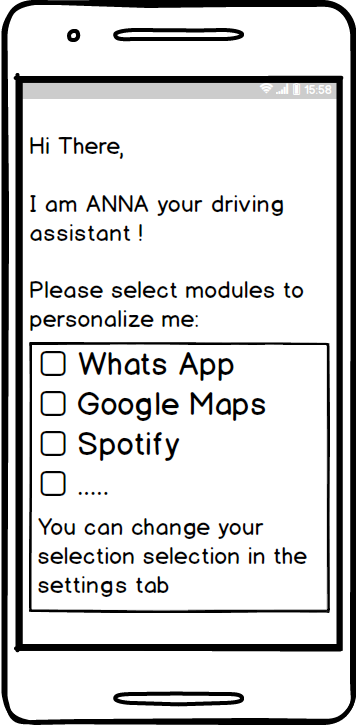
\includegraphics[scale=0.5]{images/initScreen.png}
	\caption{Initiale View}
	\label{figInitView}
\end{figure}

\subsection{Chatview}
Die Chat View verwaltet sämtliche eingehende und ausgehende Nachrichten, um den Fokus auf die Straße zu lenken. Hierbei werden eine Vielzahl von modernen Messengern unterstützt wie beispielsweise Whats App, Allo, Hangouts, Signal, Wire, Messenger und viele weitere. 

Für eine klare Strukturierung der verschiedenen Nachrichtenverläufe wurden sogenannte Cards benutzt, welche ein anpassbares Oberflächen-Element von Android darstellen. Die Cards haben hierbei eine spezielle Struktur, wodurch sich das Element in 5 Sektionen unterteilt. Diese Sektionen sind Profilfoto, Name und Nachricht des Senders, sowie das Logo des benutzen Messengers und die eingehende Uhrzeit der Nachricht. Die beschriebene Strukturierung ist in Grafik \ref{figChatView} zu sehen. Je nach Auflösung des Bildschirms des benutzten Gerätes werden verschieden viele eingegangene Nachrichten angezeigt.

Durch die genaue Strukturierung wird stets ein guter Überblick über die View gewährleistet. Zusätzlich wird dem Nutzer die Möglichkeit gegeben auf ältere Nachrichten zu antworten, da er die Namen der Sender sehen kann. 

\begin{figure}[h]
	\centering
  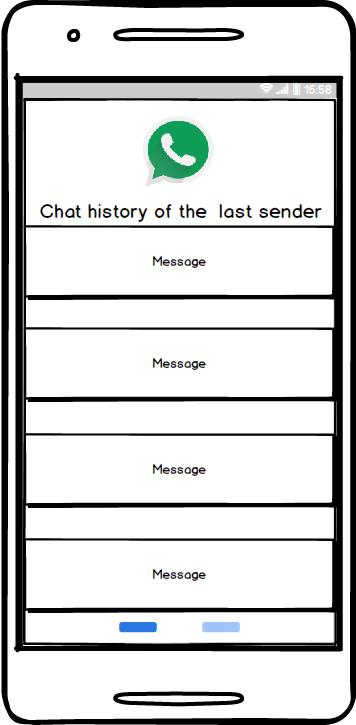
\includegraphics[scale=0.5]{images/WhatsAPP.png}
	\caption{Chat View}
	\label{figChatView}
\end{figure}

\subsection{Navigation}
Die Navigations View beinhaltet einen Navigations-Service, welcher Here Maps ist. Die Wahl des entsprechenden Services findet im Initialen Screen, \ref{figInitView}, statt. 

Nach anfänglicher Auswahl ist diese View, die standardmäßig mittlere View. Das bedeutet immer wenn die App gestartet wird, wird der Navigationsservice das erste sein, dass der Nutzer sieht. Durch die Integrierung der Applikationen wie Here Maps als Service ist es möglich alle spezifischen Funktionalitäten zu nutzen. Dies ist auf der Grafik \ref{figNavigation} zu erkennen, die einen Beispielbetrieb im Navigationsmodus des Services zeigt.

Die Spracheingabe wird jedoch über die Sprach API \ac{CMU} gehandhabt, da gewünschte Funktionalitäten nicht vorhanden sind oder Datenvolumen bereits bei der Sprachberechnung verbraucht wird. 

\begin{figure}[h]
	\centering
  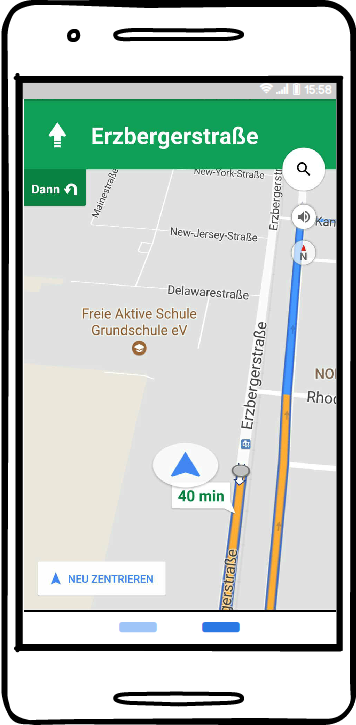
\includegraphics[scale=0.5]{images/Navigation.png}
	\caption{Navigations View}
	\label{figNavigation}
\end{figure}

\subsection{Menüführung}
Die Menüführung befasst sich mit der Navigation zwischen den verschiedenen Ansichten der Applikation. Dabei wird eine berührungslose Navigation, durch Spracheingabe und eine Navigation über den Touchscreen unterstützt.

Die berührungslose Interaktion zum Wechseln der Views, wird durch Befehle wie ,,Zeige mir die letzte View'' oder auch ,,Wechsle zur Navigationsansicht'' gesteuert. Allerdings muss der Nutzer wie bei allen anderen Befehlen das System mit dem Hotword ,,ANNA'' zunächst aus dem Schlafmodus wecken.

Im Unteren Bereich des Bildschirms befindet sich die Anzeige, welche View gerade ausgewählt ist, siehe Grafik \ref{figNavigation} und \ref{figChatView}. Dies ermöglicht eine einfache Erweiterung für neue Applikationen. Zusätzlich schafft es einen schnellen Überblick über die Anzahl der ausgewählten Module.  

Die Steuerung über den Touchscreen durch diese Anzeige sehr intuitiv. Das bedeutet, der Benutzer muss lediglich in die Richtung wischen, in der sich die gewünschte View befindet.

Befindet sich der Nutzer bereits in der am weitesten links befindlichen Ansicht und wischt dann erneut nach links öffnet sich das Einstellungsmenü. Diese Funktionalität ist in Grafik \ref{figSettings} zu sehen. In dieses Menü kann der User zusätzlich über eine Spracheingabe gelangen. Innerhalb des Menüs können Module konfiguriert und Accounts für beispielsweise Spotify oder andere Applikationen, welche Anmeldeinformationen benötigen, verwaltet werden.

\begin{figure}[h]
	\centering
  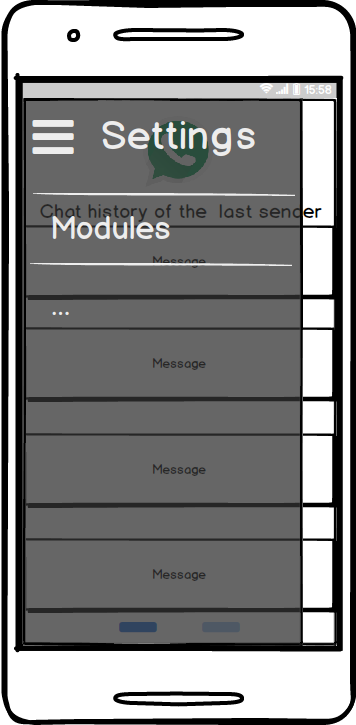
\includegraphics[scale=0.5]{images/Settings.png}
	\caption{Einstellungs View}
	\label{figSettings}
\end{figure}

\subsection{Voice Recognition}
Um das Ziel der Applikation, den Fokus wieder auf die Straße zu lenken, zu erreichen, ist die berührungslose Interaktion unabdinglich. Deshalb nimmt die Spracherkennung auch in der Oberfläche eine wichtige Rolle an. Daraus leitet sich ab, dass der Nutzer Visualisierungen für die Aufnahmefähigkeit des Gerätes und die bereits erkannte Eingabe benötigt.

Diese Visualisierung ist in Grafik \ref{figRecognition} zusehen. Um zu der beschriebenen Ansicht zu gelangen, muss der Benutzer die Spracherkennung durch das Hotword ,,ANNA'' starten. Zusätzlich zur visuellen Bereitschaftsanzeige, siehe Grafik \ref{figRecognition}, bekommt der Nutzer ein auditives Signal um dem Nutzer zu zeigen, dass \ac{ANNA} nun auf seine Spracheingaben reagiert. Dieses Signal kann je nach Einstellungen des Benutzers entweder ein einfacher Ton sein oder eine Sprachausgabe von \ac{ANNA} wie ,,Was kann ich für dich tun'' sein.
Zur Überprüfung der Eingabe kann der Nutzer sich das Gesagte vom System vorlesen lassen. Allerdings kann auf die Überprüfung der Eingabe verzichtet werden.

Durch das Ansprechen visueller und aditiver Wahrnehmung, durch Overlay und Signalton, erkennt der Nutzer jederzeit im Straßenverkehr, ob das System auf das Hotword reagiert hat und sich im Aufnahmemodus befindet, ohne dabei übermäßig abgelenkt zu werden.  
\begin{figure}[h]
	\centering
  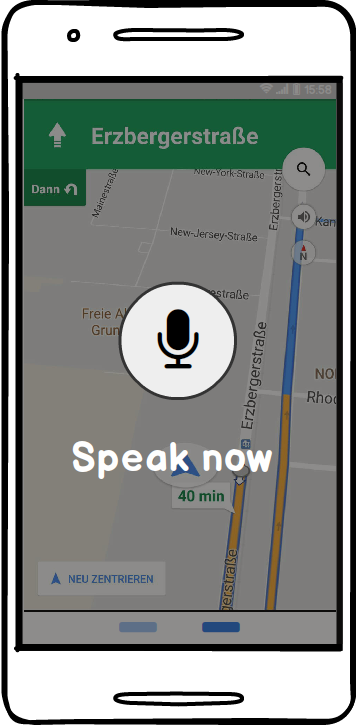
\includegraphics[scale=0.5]{images/voiceRecognition.png}
	\caption{Recognition Overlay}
	\label{figRecognition}
\end{figure}


\section{Modularität}
Bei der Umsetzung des Projekts \ac{ANNA} steht vor allem die Individualität der Nutzer im Vordergrund. Viele Dienste binden den Nutzer an die Verwendung der bereits verknüpfter Applikationen, ohne die Chance zu haben diese aus dem \ac{UI} zu entfernen oder andere vom User bereits benutzte externe Applikationen hinzuzufügen.\\
\ac{ANNA} spiegelt jedoch die Individualisierung der Nutzer wieder. Daher wird der Nutzer bei der erstmaligen Verwendung der Applikation dazu aufgefordert aus einer Liste von Applikationen diejenigen auszuwählen, die er selbst häufig benutzt und deren Unterstützung er sich von seinem persönlichen Fahrassistenten wünscht.\\
Die nach der Auswahl der Applikationen folgenden Benutzeroberflächen werden anschließend auf Basis der vom Nutzer getroffenen Modulwahl generisch zusammengestellt. Dabei ist es wichtig, dass die einzelnen Module unabhängig voneinander agieren, da eine Bereitstellung einzelner Module sonst nicht möglich wäre.

\subsection{Identifizierung externer Applikationen}
\label{installedApps}
Für das Auffinden installierter Applikationen, welche dem Nutzer über den Initial Screen zur Auswahl präsentiert werden, werden zwei verschiedene Methoden genutzt.

Innerhalb der Applikation \ac{ANNA} wird eine Liste mit den Namen der unterstützten Messengers geführt. Bei der Initialisierung der Applikation, werden zunächst alle installierten Apps, mithilfe des von Android bereitgestellten Packagemanager, abgerufen. Zusätzlich ist es mit dem Packagemanager möglich, die Namen der installierten Apps und deren Logos abzurufen. Nachdem die Informationen über die auf dem Geräte installierten Anwendungen zur Verfügung stehen wird überprüft, ob sie in der Liste enthalten sind. Wenn dies der Fall ist, wird ein entsprechendes Objekt instantiiert, welches die dazugehörige Applikation repräsentieren soll. Zu diesem Zweck werden innerhalb des jeweiligen Objektes Metainformationen zur korrespondierenden Anwendung bereitgestellt.

Bei Applikationen aus anderen Kategorien wie beispielsweise der Telefon- oder SMS-App wird ein anderer Ansatz genutzt, um dazugehörigen Anwendungen zu identifizieren.\\
Wie auch bei anderen Betriebssystemen wie beispielsweise Microsoft Windows, gibt es Applikationen die für bestimmte Zwecke oder Formate als Standard zur weiteren Verarbeitung verwendet werden. Dies ist auch bei Android der Fall. Über die Angabe einer bestimmten Kategorie wie beispielsweise \texttt{CATEGORY\_APP\_MESSAGING}, ist es möglich die jeweilige Standard Applikation für die entsprechende Kategorie abzufragen und die dazugehörigen Informationen über den Packagemanager zu erhalten.

\section{Sprachverarbeitung}
\label{languageProcessing}
Eine der wichtigsten Funktionen von Projekt \ac{ANNA} ist die Sprachverarbeitung. Sie ist die primär fokussierte Schnittstelle zur Interaktion zwischen System und Nutzer.

In den nachfolgenden Sektionen werden die einzelnen Bestandteile der Applikation, welche mit Sprachverarbeitung im Zusammenhang stehen sowie die Theroie die hinter der Sprachverarbeitung steht, näher erläutert.

\subsection{Decoding}
Zur Umwandlung von Sprache zur Text wird im Rahmen von \ac{CMU} eine statistische Modellierung namens Hidden Markov Models in Kombination mit Algorithmen verwendet. Ein Markov Model definiert sich dadurch, dass es aus n Zuständen besteht, welche jedoch nicht direkt beobachtet werden können. Dabei emmitiert jeder dieser Zustände zu jedem Zeitpunkt einen zufällig sichtbaren Zustand. Innerhalb der Spracherkennung bietet sich das Hidden Markov Model als mathematische Formulierung besonders in 2 Teilbereichen an. \footcite[vlg.:][S. 1 f.]{hmmIsolated}

Zum einen für ,,Isolated Words'' und zum andern für ,,Continous Speech''. Wie der Name beschreibt, werden bei ,,Isolated Words'' die Wörter einzeln nacheinander getrennt von einer Pause erkannt. Die genaue Berechnung des Wortes ist in Grafik \ref{figIsoRecognition} zu sehen. Dabei wird das eigehende Sprachsignal qunatisiert und somit in Vektoren zerlegt. Da jedes Hidden Markov Model ein Wort representiert wird mit Hilfe eines Algorithmus die Wahrscheinlichkeit ausgerechnet, dass die eingegange Sprachsequenz von einem dieser Model stammt. Das Model, bei dem die höchste Wahrscheinlichkeit besteht, dass die Sequenz von diesem stammt wird ausgewählt und ausgegeben.
\footcite[vlg.:][S. 12 f.]{hmmIsolated}

,,Continous Speech'' Spracherkennung ist jedoch deutlich schwerer, da der Computer im Gegensatz zur ,,isolated recognition'' nicht durch eine Pause signalisiert bekommt, dass das Wort zu Ende ist. Dies bedeutet, dass der Computer selbst entscheiden muss, wann das Wort geendet hat und wann ein neues anfängt. Allerdings ist gerade diese Entscheidungsfähigkeit des Computers unabdinglich im Hinblick auf die Spracherkennung im Projekt, da die Sprachkommandos aus zusammengesetzten Wörtern bestehen.
Im Gegensatz zur Einzelworterkennung repräsentiert wird nicht jedes Wort von einem einzelnen Hidden Markov Model zugeordnet, sondern es wird ein großes Model gebaut, durch das hinzufügen von Übergangszuständen. Spracherkennung auf Basis dieses neu erzeugten Models, funktioniert nun durch das Suchen nach der Sequenz an Zuständen, welche am wahrscheinlichsten mit der Sequenz des gegebenen Beobachtungsvektor übereinstimmt. Diese Wahrscheinlichekiten werden über einene Algorithmus bestimmt. 
\footcite[vlg.:][S. 29 f.]{hmmContinous}

\begin{figure}[h]
	\centering
  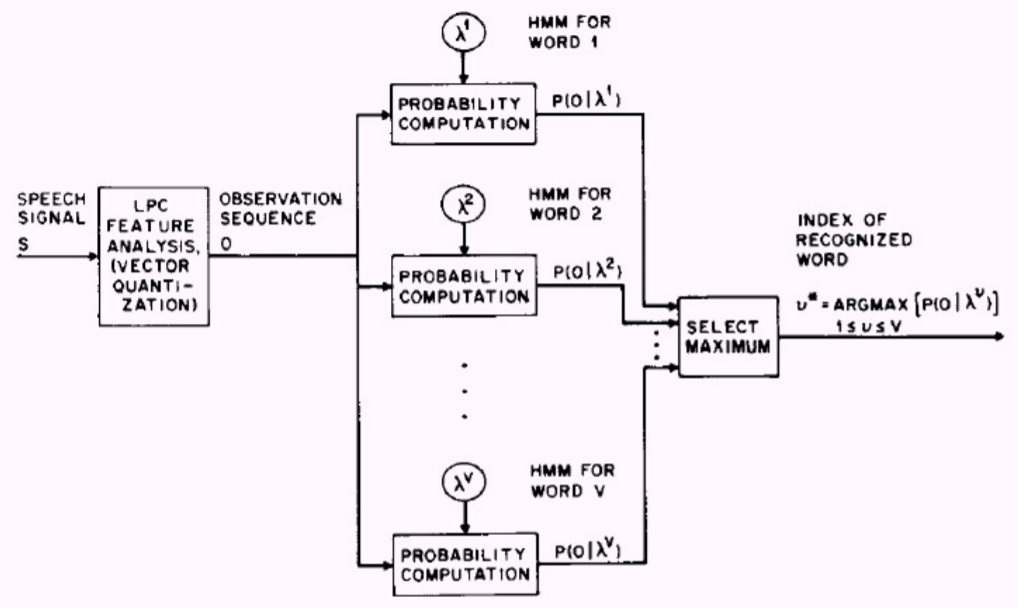
\includegraphics[scale=0.5]{images/iso_word_recog.png}
	\caption{Isolated Word Recognizer}
	\label{figIsoRecognition}
\end{figure}


\subsection{Störgeräuschreduktion}
In einem Sprachsignal sind immer Hintergrundgeräusche enthalten. Diese Hintergrundgeräusche maskieren das eingehende Signal derart, dass Qualitätsverluste die Folge sind. Wenn das Sprachsignal ohne eine Störgeräuschreduktion prozessiert werden würde, wäre die Performance des Systems erheblich schlechter, da dieses falsch Interpretationen aufgrund von Störgeräuschen zusätzlich berechnen würde.
Um diesen Performanceverlust entgegenzuwirken und um eine klareres Bild des Signals zu bekommen, gibt es spezielle Lärmunterdrückungs-Algorithmen. 
\footcite[vlg.:][S. 1 ]{specSub}

Einer dieser Algorithmen ist der, der spektralen Subtraktion. Die spektrale Subtraktion ist den Einzel-Kanal-Sprachverbesserungen zugehörig. Im Gegensatz zur Mehrfach-Kanal-Sprachverbesserung kann mit wenig Aufwand eine akzeptable Trennung von Sprache und Lärm innerhalb eines Signals erreicht werden. Die spektrale Subtraktion findet auch in \ac{CMU}, zur Reduzierung von Hintergrundgeräuschen, Verwendung. 
\footcite[vlg.:][S. 1 ]{specSub}

Um die Störgeräusche herauszufiltern stützt sich die spektrale Subtraktion auf die Formel \ref{noiseSum}. Hierbei setzt sich das unklare, geräuschvolle Signal u(s) aus dem eingehenden Sprachbefehl c(s) und den Hintergrundgeräuschen n(s) zusammen. Um den klaren Sprachbefehl zu bestimmen, wird n(s) geschätzt und vom Signal abgezogen. 
\footcite[vlg.:][S. 2 f.]{specSub}

%\begin{equation}
%    \label{noiseSum}
%    u(s) = c(s) + n(s) 
%\end{equation}

Der Ablauf des Algorithmus ist in Grafik \ref{figspecSub} zu sehen. 
In diesem Fall wird ein unklares, geräuschvolles Signal in meherere kleine Frames zerteilt. Danach wird mit Hilfe der Schnellen Fouriertransformation das Signal in den Frequenzraum transformiert, da sich dort mathematische Operationen leichter anwenden lassen. Die Diskrete Kosinus Transformation wird wiederum dazu genutzt, um die Urpsrungstöne zu finden, welche durch Überlagerungen von Tönen entstanden. Durch die Berechnung der Ursprungstöne und die Analyse der einzelnen Frames kann eine Abschätzung des Hintergrundgeräusches vorgenommen werden. Die Analyse der einzelnen Frames ist unabdinglich, da Frames existieren bei denen zum Zeitpunkt t kein Signal vom Nutzer eingeht und somit das Signal als Hintergrundgeräusch gedeutet werden kann.
Ausgehend von den Berechnungen wird nun ein gewisser Prozentsatz des Hintergrundgeräusches ne(w) vom Eingangssignal m(w) abgezogen. Um nun zu c(s) aus Formel \ref{noiseSum} zugelangen, muss das Signal wieder zurück transformiert werden. Nun steht dem Decoding des eigegangenen Signals nichts mehr im Weg.
\footcite[vlg.:][S. 2 f.]{specSub}
\footcite[vlg.:][]{fft}
\footcite[vlg.:][]{dct}

\begin{figure}[h]
	\centering
  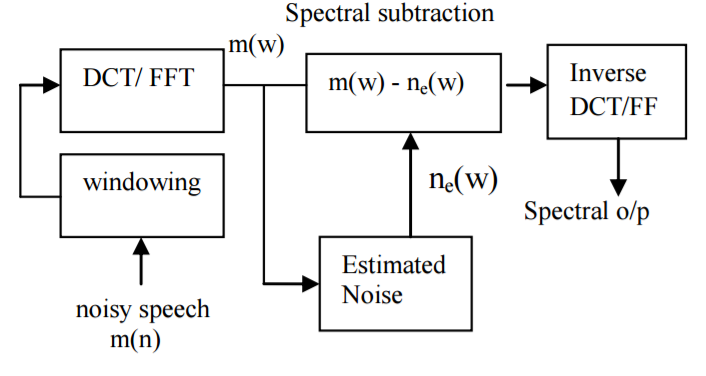
\includegraphics[scale=0.7]{images/spectral_sub.png}
	\caption{Sequenz Diagramm der Spektralen Subtraktion}
	\label{figspecSub}
\end{figure}

\subsection{Spracherkennung}
Die Erkennung der gesprochenen Sprache erfolgt anhand der durch den User eingestellten Systemsprache des Geräts.\\
Bei der Initialisierung der Speech Engine wird zunächst, über eine von Android bereit gestellte Funktion, die eingestellte System Sprache abgefragt, um anhand dieses Ergebnisses die entsprechenden Sprachbibliotheken und definierten Grammatiken zu laden.\\
Für den Nutzer bietet dies den Vorteil sich nicht mit zusätzlichen Einstellungen beschäftigen zu müssen und ein besseres Ergebnis bei der Sprach in Textumwandlung zu erhalten. Diese Vorgehensweise hat jedoch auch einen negativen Aspekt. Da die Systemsprache eindeutig ist und es beim aktuellen Stand nicht möglich multilingual mit dem System zu interagieren. Eine Eingabe in einer Sprache, welche nicht der Systemsprache entspricht, erzielt somit weniger bis gar keine genauen Ergebnisse bei der Umwandlung in Text.

Um den benötigten Speicher sowie die Komplexität im Rahmen dieser Studienarbeit gering zu halten, bietet die Spracherkennung zunächst nur die Erkennung für die Sprachen Deutsch und Englisch an.\\
Je nach voranschreiten der Entwicklung und der verbleibenden Zeit werden weitere Sprachen unterstützt.

\subsection{Hotword Detection}
\label{scthotword}
Um das Ziel der Reduzierung von Verkehrsunfällen durch Smartphone Interaktionen zu minimieren, ist es wichtig jegliche Berührung des Smartphones und der damit verbundenen Ablenkung vom Straßenverkehr zu reduzieren.\\
Die in diesem Kapitel beschriebenen Spracherkennungsfunktionen sind ein wichtiger Schritt hin zur Erfüllung dieses Ziels.\\1
Viele Speech-to-Text Dienste funktionieren an dieser Stelle auf die Weise, dass der Nutzer zunächst einen Knopf betätigen muss um die Sprachaufnahme und die damit verbundenen Umwandlung in Text zu starten. Bei einigen Tools ist es sogar notwendig für die Dauer der Sprachaufnahme den entsprechenden Knopf gedrückt zu halten.\\
Ein solches Verfahren ist für Projekt \ac{ANNA} eher ungeeignet, da der Nutzer des öfteren den Blick von der Straßen weg hin zu seinem Smartphone richten müsste um den entsprechenden Knopf ausfindig zu machen und diesen zu drücken.\\
Um dieses Problem zu umgehen, kommt an dieser Stelle eine Hotword Detection zum Einsatz.

Als Hotword Detection bezeichnet man die Suche nach einem bestimmten Wort oder einem kurzen Satz in einem kontinuierlich aufgenommenen Audiostream.\\
Hierzu wird sobald die Applikation gestartet wurde und die erstmalige Initialisierung abgeschlossen ist, die Speech-to-Text Engine initialisiert und kontinuierlich alle eingehenden Audiosignale auf das Auftreten des definierten Hotword geprüft.\\
Wird das Hotword nicht erkannt, werden die Aufnahmen ohne weiter Verarbeitung verworfen. Sobald jedoch das Hotword erkannt wurde, startet die interne sprachbasierte Menüführung zur Identifikation der vom Nutzer gewünschten Aktion. Weitere eventuell benötigte Informationen werden über einen Dialogmodus, im Sinne von Frage durch das System und Antwort des Nutzers, in Erfahrung gebracht.

\subsection{Kontext basierte Grammatiken}
Betrachtet man die reale Welt, bemerkt man schnell, dass die Reihenfolge sowie die Anzahl der sinnvoll zu verwendeten Wörter durch die jeweilige Situation eingeschränkt sind. Diese Erkenntnis lässt sich auch bei der Spracherkennung anwenden.\\
Betrachtet man zum Beispiel folgendes Szenario: Ein Nutzer möchte ein Telefonat führen und diktiert die Telefonnummer die er anrufen möchte. Da Telefonnummern nur aus Zahlen bestehen und gegebenenfalls aus einem Plus für die Landesvorwahlen, lässt sich der Umfang der für die Speech-to-Text Engine zu prüfenden Wörter entsprechend auf Zahlen reduzieren, wodurch die Genauigkeit der erfolgreichen Speech-to-Text Umwandlung erhöht wird.

Die Einschränkung der zu überprüfenden Wörter erfolgt hierbei durch die Definition verschiedener Grammatiken, welcher in einer Backus-Naur ähnlichen Form definiert werden.\\
Die so definieren Grammatiken können dann je nach Kontext in dem sich der User durch seine vorherige Spracheingabe befindet geladen werden, um die jeweilige Genauigkeit bei der Spracherkennung zu erhöhen.\\
Zur Veranschaulichung der Struktur einer solchen Grammatik, zeigt Listing \ref{lstGrammar} eine simple Grammatik zur Erkennung einer einfachen Telefonnummer. Die für CMU Sphinx verwendeten Grammatiken werden dabei alle in \ac{JSGF}-Dateien definiert.

\begin{lstlisting}[caption={Einfache Grammatik zur Erkennung von Telefonnummern},captionpos=b,label=lstGrammar]
#JSGF V1.0 ISO8859-1 de;

grammar call;

public <number> = <digit>*;
<digit> = eins | zwei | drei | vier | fünf | sechs | sieben | acht | neun | null;
\end{lstlisting}

\section{Benachrichtigungsverarbeitung}
Zur Reduzierung der Ablenkung des Nutzers während der Fahrt durch neue Benachrichtigungen auf dem Smartphone, werden diese abgefangen und dem Nutzer auf Wunsch vorgelesen und die Möglichkeit geboten direkt auf diese zu antworten.

Um neue Benachrichtigungen abzufangen wird ein Notification Listener instanziiert. Damit dieser Zugriff auf eingehende Benachrichtigungen erhält, muss der Nutzer zunächst die entsprechende Einstellung an seinem Smartphone durchführen. Zur Erleichterung dieses Schrittes, wird der Nutzer während der erstmaligen Inbetriebnahme der Applikation durch die nötigen Konfigurationsschritte geführt.

Nach der erfolgreichen Konfiguration und der Gewährung aller nötigen Berechtigungen, ist der Notification Listener bereit neue Benachrichtigungen abzufangen und die Applikation ist somit in der Lage, den in Graphik \ref{figNotification} dargestellte Programmablauf auszuführen. Geht eine neue Benachrichtigung am Smartphone ein, wird per Broadcast an alle registrierten Notification Listener gesendet. Diese bieten, da sie von der abstrakten Klasse \texttt{NotificationListenerService} erben, verschiedene Methoden welche bei einer Veränderung des Status einer Benachrichtigung aufgerufen werden. Mögliche Beispiele wären hier die Methoden \texttt{onNotificationPosted}, welche aufgerufen wird wenn eine neue Benachrichtigung im System eingeht oder die Methode \texttt{onNotificationRemoved}, die beim Entfernen einer Benachrichtigung aufgerufen wird.

Stellt der Notification Listener fest, dass eine neue Benachrichtigung vom System eingegangen ist, prüft die Applikation zunächst ob es sich beim Erzeuger der Benachrichtigung um eine Applikation handelt, welche vom Nutzer als Modul aktiviert wurde. Trifft dieser Fall ein, wird die Benachrichtigung vom System abgerufen und zunächst zur besseren Verarbeitung in ein applikationsinternes Datenformat transformiert. Anschließend wird dem Nutzer mittels Text-to-Speech Engine der Titel der Benachrichtigung vorgelesen. Bei dem Titel einer solchen Benachrichtigung handelt es sich um Informationen, die benötigt werden um den restlichen Inhalt einer Benachrichtigung zuordnen zu können. Bei einer eingehenden WhatsApp Nachricht, würde dieser Titel wie folgt lauten: Eine neue Nachricht von Max Mustermann.\\
Der Nutzer wird anschließend wiederum per Text-to-Speech Mechanismus gefragt ob er den Inhalt der Nachricht vorgelesen bekommen möchte. Die Antwort des Nutzers wird dann wiederum per Speech-to-Text Engine umgewandelt. Sollte das Ergebnis dieser Antwort positiv sein, wird die Nachricht vorgelesen und der Nutzer weiterhin gefragt ob er auf diese Nachricht antworten möchte.\\
Für die Text-to-Speech Umwandlung wird einfachheitshalber die vom Nutzer primär eingestellte Text-to-Speech Engine verwendet. Für die Auswertung der Antworten des Nutzers wird das Framework CMU Sphinx verwendet, welches in Sektion \ref{sctcmu} näher beschrieben wird.

\begin{figure}[h]
	\centering
  \includegraphics[scale=0.5]{images/notification.png}
	\caption{Ablaufsdiagramm für den Eingang einer neuen Benachrichtigung}
	\label{figNotification}
\end{figure}

Die Vorlesefunktion neuer Benachrichtigung funktioniert mit jeder gängigen Applikation, da es sich bei dem Abfangen neuer Benachrichtigungen um eine Android spezifische Standardfunktion handelt.\\
Gerade bei Messenger Diensten, variiert jedoch die Offenheit der Messenger gegenüber der Nutzung durch dritte. Einige Dienste bieten hier eigene \ac{API}s an um mit den Messenger Dienst zu interagieren, andere wie beispielsweise der populäre Dienst WhatsApp jedoch, bieten keinerlei offizielle Schnittstelle für die Nutzung durch dritte.\\
Um den Entwicklungsaufwand an dieser Stelle in einem vertretbaren Maße zu halten und gleichzeitig möglichst viele Messenger zu unterstützen ohne, dass selbst der exotischste Messenger bekannt sein muss, wird an dieser Stelle ein Workaround angewendet.\\
Mit der Einführung von Android Wear und den damit erschienen \gls{Wearables}, entwickelte Google eine neue Datenstruktur, welche speziell für das anzeigen und Antworten über Wearables konzipiert ist. Diese Datenstruktur enthält eine Referenz, welche es ermöglicht gezielt auf eine neue Nachricht von einem bestimmten Kontakt aus dem jeweiligen Messenger zu antworten. Diese neue Datenstruktur, welche als \texttt{WearableExtender} bezeichnet wird, wird im Benachrichtigungsobjekt referenziert.\\
Geht nun eine neue Benachrichtigung ein, wird das \texttt{WearableExtender} Objekt, welches normalerweise an ein Wearable Gerät gesendet werden würde aus dem Benachrichtigungsobjekt extrahiert und für die direkte Interaktion mit den jeweiligen Messenger und speziell mit dem jeweiligen Kontakt verwendet.\\
Deshalb ist es nicht mehr erforderlich die Unterstützung für jeden Messenger einzeln zu implementieren und sich mit deren Funktionsweise auseinanderzusetzen.

	\chapter{Evaluation der finalen Applikation}

In diesem Kapitel wird die Dashboard Applikation anhand zahlreicher verschiedener Kriterien Evaluiert. Der Großteil dieser Kriterien wurde zuvor in der Sektion \ref{sec:requirements} vereinbart. Dazu zählen Offline Verfügbarkeit, Modularität, Hotword Detection, Qualität der Spracherkennung und Ausgabe, Navigation, Anrufen, SMS, Messenger Integration, Musik Dienste, Nachtmodus, die Bedienung des Geräts ausschließlich über Sprache und ein übersichtliches Design.

Die Offline Verfügbarkeit der Applikation wird durch die Verwendung der Speech \ac{API} \ac{CMU} erreicht, welches durch die Verwendung von selbst definierten Grammatiken einen Performance Steigerung bietet. Zusätzlich wird durch die Kontext Spezifizierung eine Erhöhung der Sprachqualiät und durch Verwendung von \ac{VA} eine gute Sprachausgabe erreicht. Jedoch wird eine Nachjustierung der Parameter notwendig werden, da sich der Kontext mit jeder externen Applikation vergrößert und eine Erkennungsrate von mindestens 90 Prozent wie in Kapitel \ref{chpt:Mic} beibehalten werden soll.  

Das Konzept der Modularität der Applikation zieht sich die komplette Applikation. Dies fängt breits beim ersten Starten der App an, in dem sich der Nutzer \ac{ANNA} personalisieren kann. Weiterhin kann der Benutzer unabhängig von seiner bisherigen Auswahl an Modulen diese jederzeit in den Einstellungen ändern und an seine Bedürfnisse anpassen. Das Ergebnis dieser Modularität kann in Grafik \ref{figANNAStatusbar} betrachtet werden, wobei einmal alle zur Verfügung stehenden Funktionen ausgewählt wurden und einmal nur die vom Nutzer benötigten. 

\begin{figure}[h]
	\centering
  
\includegraphics[scale=0.5]{images/status_bars.png}
	\caption{Nutzer ausgewählte Module für \ac{ANNA}}
	\label{figANNAStatusbar}
\end{figure}

Das Kriterium der ausschließlichen Bedienung über Sprache wird mit Hilfe der Hotword Detection gelöst, wodurch \ac{ANNA} stehts über das Hotword ,,Hey ANNA'' aktiviert werden kann und somit auf die Eingaben des Nutzers hört. Dadurch können wie im Laufe der Arbeit beschrieben Kontakte angerufen, Navigationsziele festgesetzt, zwischen den Views gewechselt, auf Nachrichten reagiert und Musiktitel, welche sich lokal auf dem Smartphone befinden, abgespielt werden.

Für die Navigation des Nutzers, unabhängig von seinem Standort, wird das Open Source SDK Here Maps verwendet, welches sich durch seine vollständige Konfigurierbarkeit in das Konzept der Applikation perfekt integrieren lies. Here Maps bietet aufgrund umfassender Karten und Datenbank Anbindungen viele Optionen zur Verbesserung des Fahrempfindens an, wie beispielsweise Stauumfahrung und Geschwindigkeitsanzagen.

Weiterhin kann der Nutzer während einer Fahrt durch einen Sprachbefehl Personen aus seiner Kontaktliste anrufen, damit die Aufmerksamkeit durchgehend auf die Straße gerichtet und nicht durch das Heraussuchen eines Kontaktes vermindert wird.

Zur Entgegenwirkung der größten Ablenkung, eingehende Nachrichten jeglicher Messenger, unterstüzt \ac{ANNA} eine Vielzahl von aktuellen Nachrichtendiensten. Zu diesen zählen unter anderem Whats App, Signal, Hangouts, Wire, Allo und weitere. Außerdem werden auch altmodische Nachrichten Dienste wie SMS unterstützt. Durch die Annahme und Beantwortung per Sprache kann somit eine deutlich erhöhte Fokusssierung auf den Straßenverkehr erreicht werden. Allerdings wird der Dialog mit \ac{ANNA} bei eingehenden Nachrichten durch laute Umgebungsgeräusche erheblich erschwert, wenn eine gewissen Grenze überschritten wird, welche nach verschiedenen Tests bei knapp 90 Dezibel liegt. 

Damit auch die Musikauswahl während der Fahrt nicht weiter ablenkt, wurde der Android Musicplayer integriert. So kann der Nutzer Wunschlieder äußern und bei nicht gefallen eines Liedes zum nächsten oder zum vorherigen springen. Vorraussetzung dafür ist jedoch das vorliegen der Musik auf dem Smartphone, da weitere Musikdienste nicht eingebunden sind. 

Zur angenehmen Bedienung der Applikation wurde auf ein übersichtliches und schlichtes Design gesetzt, um dazu beizutragen den Benutzer während der Fahrt nicht abzulenken. Des weiteren wird durch die Verwendung eines speziellen Nachtmodus auch bei Nachtfahrten ein angenehmes Empfinden der Helligkeit im Fahrzeug erreicht. Dies wird durch das Wechseln der Farben von hell zu dunkel erreicht, welches durch die automatische Anpassung der Bildschirmhelligkeit durch das Betriebssystem zusätzlich verbessert werden kann.  


	\chapter{Fazit}
Bei der Entwicklung der Applikation \ac{ANNA} spielten sowohl Erfahrungen als auch neue Erkenntnisse eine zentrale Rolle.\\
Durch den Vergleich mit bestehenden Produkten kristallisierte sich ein guter Fokus für die Entwicklung der Anwendung heraus. Zusätzlich wurden durch die immer wieder durchgeführten Tests der Applikation in realistischen Nutzungsumgebungen Schwachstellen erkannt und diese umgehend behoben. So wurde beispielsweise als Ergebnis eines solchen Tests die Benutzeroberfläche von Grund auf neu gestaltet. So wurde sichergestellt, dass die einzelnen Elemente auch auf einer mittleren Distanz, wie sie während der Fahrt herrscht wenn das Smartphone sich in einer entsprechenden Halterung befindet, gut zu erkennen sind.

Auch konnten während der Entwicklung Erfahrungen zum Umgang mit Spracherkennugsframworks und deren Probleme hinsichtlich der Verwendung in einer Anwendung wie \ac{ANNA} gesammelt werden.\\
Beispielsweise stellte sich so die Problematik der Verwendung der Spracherkennung während der Nutzung eines Musik-Players heraus.

In Anbetracht des begrenzten Entwicklungszeitaums, konnten einige Funktionen nur in begrenzten Umfang umgesetzt werden, woraus sich die in Kapitel \ref{ausblick} beschriebenen weiteren Entwicklungsspielräume ergeben.\\
Dennoch ist mit dem Ergebnis dieser Arbeit bereits eine Lösung entstanden, mit deren Hilfe sich die Ablenkung im Straßenverkehr durch Smartphones reduzieren lässt.

Generell lässt sich sagen, dass durch die Entwicklung dieses Projekts viele neue Erkenntnisse zu mobilen Plattformen, Spracherkennungsfunktionen, Mensch-Computer Interaktionen und der Gestaltung von Benutzeroberflächen sammeln ließen. Außerdem wurde ein nicht unwesentlicher Beitrag zur Reduzierung von Verkehrsunfällen geleistet, welcher im besten Fall sogar Menschenleben retten kann. 
	\chapter{Ausblick}
\label{ausblick}
Die Entwicklung des Projekts \ac{ANNA} hat bereits einen guten Stand erreicht, jedoch gibt es noch Verbesserungspotential für die zukünftige Entwicklungsarbeit.

Aus technischer Sicht kann die Applikation zukünftig verbessert werden, indem Optimierungen an der Performance vorgenommen werden.\\
Einige Funktionen die durch die Applikation bereitgestellt sind äußerst Zeitaufwändig. Eine mögliche Verbesserung wäre es an dieser Stelle die entsprechenden zeitkritischen Programmteile zu parallelisieren, um so eine bessere Geschwindigkeit bei der Erfüllung der gebotenen Funktionen zu erreichen und dem Benutzer ein flüssigeres Nutzererlebnis zu liefern.\\
Als konkretes Beispiel für einen solch zeitkritischen Programmteil ist hier die Einrichtung der Applikation nach dem erstmaligen Start abzuführen.

Ein weiteres Verbesserungspotential verbirgt sich hinter den Spracherkennungsfunktionalitäten.\\
Da das bei der Entwicklung verwendtete Framework, \ac{CMU} in erster Linie für die englische Sprache entwickelt wird, ist die Anzahl der im phonetischen Wörterbuch enthaltenen Wörter der deutschen Sprache eher gering. Hieraus ergibt sich der Bedarf der Erweiterung des verwendeten Wörterbuchs, um so die Spracherkennung zu verbessern.\\
Zusätzlich wäre es möglich den Nutzer die verwendeten Grammatiken personalisieren zu lassen, so dass sich für die Verwendung der Spracherkennungsfunktionen ein natürlicheres Konversationsgefühl ergibt. Zusätzlich würde diese Konfiguration die Möglichkeiten der personalisierung der Applikation weiter erhöhen.\\
Denkbar wäre es hier zum Beispiel, dass dem Nutzer der Sprachbefehl "navigiere mich nach...", welcher zum starten der Turn-by-Turn Navigation verwendet wird, nicht gefällt. Durch die neue Konfigutarionsmöglichkeit könnte er den Befehl dann zum Beispiel zu "bring mich nach..." umwandeln.

Aus Funktionsumfangtechnischer Sicht ergeben sich für zukünftige Entwicklungen die Möglichkeit mehr Dienste in die Applikation zu integrieren. Möglich wäre es hier beispielsweise aus Sicht der Messenger Anwendungen die Liste der unterstützten Messenger zu erweitern und ebenfalls nicht nur die Möglichkeit zur Antwort auf einen Chatt zu bieten sondern auch die Möglichkeit einen neune Chatt zu initialisieren.\\
Auch aus Sicht der Musik-Diensten würden sich weitere Dienste implementieren lassen und so wäre es möglich dem Nutzer noch wesentlich größere Personalisierungsmöglichkeiten zu bieten.

Auch bei dem angebotenen integrierten Navigationsdienst besteht die Möglichkeit noch weitere Dienste in die Applikation zu implementieren und die durch den Navigationsdienst bereitgestellten Funktionen zu erweitern.\\
Beispielsweise ist es denkbar, dass in Zukunft neben der reinen Turn-by-Turn Navigation zusätzliche nützliche Funktionen wie beispielsweise eine Blitzerwarnung, die Anzeige von Geschwindigkeitslimits oder das suchen nach \ac{POI} zur Verfügung stehen.\\
Außerdem wäre es denkbar den Nutzer die Darstellung der Navigationfunktion, über den Einstellungsbereich der Applikation, stärker an seine Vorlieben anzupassen. Zum Beispiel wäre es so für den Nutzer möglich die Ansicht zwischen 2D und 3D zu wechseln.

	\chapter{Anhang}

\section{Benutzeranleitung}
	
	% Anhang
	\clearpage
	\pagenumbering{roman}

	% Abbildungsverzeichnis
	\cleardoublepage
	\phantomsection \label{listoffig}
	\addcontentsline{toc}{chapter}{Abbildungsverzeichnis}
	\listoffigures

	%Tabellenverzeichnis
	\cleardoublepage
	\phantomsection \label{listoftab}
	\addcontentsline{toc}{chapter}{Tabellenverzeichnis}
	\listoftables

	% Quellcodeverzeichnis
	\cleardoublepage
	\phantomsection \label{listoflist}
	\addcontentsline{toc}{chapter}{Listings}
	\lstlistoflistings

	% Literaturverzeichnis
	\cleardoublepage
	\phantomsection \label{listoflit}
	\addcontentsline{toc}{chapter}{Literaturverzeichnis}
	
	%Bib style
	%\bibliographystyle{agsm} %Havard
	%\bibliographystyle{amsplain} %Durchnummeriert
	%\bibliographystyle{amsalpha} %Kürzel für Autor und Jahr
	%see more: http://amath.colorado.edu/documentation/LaTeX/reference/faq/bibstyles.pdf
	
	%\bibliography{ArbeitBib}
	\printbibliography[title={Literaturverzeichnis}]
	
	% Abkürzungsverzeichnis
	\cleardoublepage
	\phantomsection \label{listofacs}
	\addcontentsline{toc}{chapter}{Abkürzungsverzeichnis}
	%!TEX root = ../dokumentation.tex

\chapter*{Abkürzungsverzeichnis}
%nur verwendete Akronyme werden letztlich im Dokument angezeigt
\begin{acronym}[YTMMM]
\setlength{\itemsep}{-\parsep}

\acro{ANNA}{Auto Notification Narrator Assitent}
\acro{API}{Application Programming Interface}
\acro{CMU}{CMU Sphinx}
\acro{CS}{Google Cloud Speech}
\acro{JSGF}{JSpeech Grammar Format}
\acro{MVC}{Model View Controller}
\acro{POI}{Points Of Interest}
\acro{UI}{User Interface}
\acro{VA}{Voice Action}
\acro{VM}{Virtuelle Maschine}

\end{acronym}

	
	% Glossar
	\printglossary[style=altlist,title=Glossar]
\end{document}
